\chapter{LA SYNTAXE : L’EXPLORATION DE LA PHRASE}
\label{chapter-10}
\markright{La syntaxe}
\origpage{284}{270}
\begin{keybox}[Plan du chapitre]
\small\setstretch{1.01}
\setlist{topsep=.12em,itemsep=.12em,parsep=0pt}
\renewcommand{\thempfootnote}{校\arabic{editorialnote}}
\textbf{I.\quad LA PHRASE, OBJET LINGUISTIQUE MULTIFORME}
\begin{enumerate}[label=\arabic*.]
\item Définitions de la phrase
\begin{enumerate}[label=\textcircled{\scriptsize\arabic*}]
\item Notions de base\par
1. Différences entre Phrase et énoncé\par
2. Phrase simple et phrase complexe\par
3. Phrase enchâssante et phrase enchâssée
\item Les trois types de relation syntaxique\par
1. La coordination\par 2. La subordination\par 3. La juxtaposition
\end{enumerate}
\item La Délimitation de la phrase
\begin{enumerate}[label=\textcircled{\scriptsize\arabic*}]
\item Syntaxe débordant du cadre de la phrase
\item Phrase contenant des propositions indépendantes
\item Phrases verbales, non verbales et averbales\par
1. La phrase verbale, nœud verbal\par
2. La phrase non verbale\par
3. La phrase averbale
\end{enumerate}
\item Jugements possibles sur une phrase
\begin{enumerate}[label=\textcircled{\scriptsize\arabic*}]
\item L’agrammaticalité
\item L’asémanticité
\item L’acceptabilité
\item L’interprétabilité
\end{enumerate}
\end{enumerate}
\textbf{II.\quad LA SYNTAXE STRUCTURALE DE LUCIEN TESNIÈRE}
\begin{enumerate}[label=\arabic*.]
\item Concept et postulats de base
\begin{enumerate}[label=\textcircled{\scriptsize\arabic*}]
\item L’objet de la syntaxe structurale
\item Les deux ordres de la phrase
\item La notion de structure profonde
\item Indépendance du plan structural et sémantique
\item Le stemma
\end{enumerate}
\origpage{285}{271}
\item Le modèle dépendanciel
\begin{enumerate}[label=\textcircled{\scriptsize\arabic*}]
\item La connexion
\item La translation\par
1. Classe de mots et fonctions syntaxiques\par
\hspace{1em}1) Les mots pleins\par \hspace{1em}2) Les mots vides\par
2. Correspondance entre fonctions et catégories\par
3. Transférende, translatif, transféré\par
4. Représentation graphique\par
5. Translation, transposition et transformation
\item La jonction\par
1. La notion de dédoublement\par 2. La jonction sans jonctif\par
3. La jonction de la phrase\par 4. Le cas de l’anaphore
\end{enumerate}
\item Le schéma actantiel
\begin{enumerate}[label=\textcircled{\scriptsize\arabic*}]
\item Le verbe, « nœud des nœuds »\par
1. Du « nœud » au « nucléus »\par 2. Première définition\par 3. Deuxième définition
\item Les actants\par 1. Prime actant\par 2. Second actant et tiers actant
\item Les circonstants
\end{enumerate}
\item La notion de valence
\begin{enumerate}[label=\textcircled{\scriptsize\arabic*}]
\item L’origine de la notion
\item La valence des verbes\par
1. Les verbes avalents\par 2. Les verbes monovalents\par
3. Les verbes bivalents\par 4. Les verbes trivalents
\item La valence des noms
\item La valence des adjectifs
\end{enumerate}
\end{enumerate}
\textbf{Exercices}\par\textbf{Pour aller plus loin}\par\textbf{Glossaire}
\end{keybox}

\Needspace{8\baselineskip}
\origpage{286}{272}
\begin{keybox}[Introduction]
\renewcommand{\thempfootnote}{校\arabic{editorialnote}}
Emprunté au grec ancien {\BBSixGreek σύνταξις} \textit{súntaxis}, le mot syntaxe signifie « mise en ordre », « assemblage ». La syntaxe est donc la branche de la linguistique qui étudie la façon dont les lexèmes se combinent en syntagmes pour former des propositions qui se combinent à leur tour en phrases. Voilà pour la définition générale, mais il convient de la préciser, car de la même manière que le terme de grammaire renvoie à des démarches différentes, il existe aujourd’hui différentes approches théoriques de la syntaxe, même si elles partagent le même objet, à savoir la phrase.
\begin{itemize}
\item En grammaire traditionnelle, la syntaxe s’intéresse aux relations entre les mots qui constituent une proposition ou une phrase, à leurs combinaisons, ainsi qu’aux règles qui gouvernent ces dernières. Cette syntaxe fera l’objet de la première partie de ce chapitre.
\item La syntaxe structurale est une analyse descriptive des unités composant les énoncés et des relations hiérarchiques que ces unités entretiennent entre elles. La deuxième partie de ce chapitre sera consacrée aux travaux originaux du linguiste français Lucien Tesnière dans ce domaine.
\item L’approche la plus récente de la syntaxe est la syntaxe générative. Partie essentielle du modèle de grammaire générative (\textit{generative grammar}) de Noam Chomsky, cette syntaxe a pour fonction d’engendrer selon des règles formelles toutes les énoncés considérés comme grammaticaux.\ednote{原文 toutes les énoncés 的性配合有误，应为 tous les énoncés。} Cette syntaxe générative fera l’objet d’un développement spécifique et détaillé dans le chapitre 14.
\end{itemize}
\end{keybox}

\section{LA PHRASE : UN OBJET LINGUISTIQUE MULTIFORME}
Domaine de la linguistique consacré à la description de la phrase, la syntaxe formule des règles d’agencement des mots et groupes de mots entre pour former des phrases.\ednote{原文 entre pour 连用，句法不完整；按本句意思可校为 des mots et groupes de mots entre eux pour former des phrases，或删去 entre。正文保留原字，不将拟补 eux 当作已见原文。} Tous les linguistes s’accordent sur un point : l’unité de base de la syntaxe est la phrase. Mais ils s’accordent aussi sur un autre point : la difficulté, voire l’impossibilité de la définir.

\subsection{Définitions de la phrase}
Sur la question délicate de la définition de la phrase et l’objectif de la syntaxe, je vous invite à lire le point de vue de la linguiste française \textbf{Marie-Noëlle Gary-Prieur} (1946-) :
\begin{quote}\small\itshape
On ne peut espérer une définition qui permettrait d’opposer clairement les objets qui sont des phrases et ceux qui n’en sont pas. On peut dire que c’est l’objectif même de la syntaxe de décrire les différentes formes de phrases.
\end{quote}

\origpage{287}{273}
Il n’existe donc pas de définition unique de \textit{la} phrase : il existe \textit{des} phrases, et ce sont elles, dans leur diversité, qui constituent l’objet de la syntaxe. Avant donc de commencer à décrire plus bas les différentes formes de phrases, essayons tout de même de réfléchir à ce qu’est une phrase.

\minititle{\textcircled{\scriptsize 1} Notions de base}
Dans la 9\textsuperscript{e} édition de son \textit{Dictionnaire}, l’Académie Française définit ainsi la phrase : « Proposition simple ou ensemble de propositions, grammaticalement autonome, et qui présente une unité de sens. » La phrase est donc vue comme une entité caractérisée par une double autonomie : autonomie sémantique et autonomie syntaxique. Le contenu sémantique se dégage du rapport établi entre les signes de la phrase, mais il dépend aussi, du contexte et de la situation d’énonciation : il nous faut donc dans un premier temps établir une première distinction entre phrase et énoncé.

\minititle{1. Différence entre phrase et énoncé}
La phrase est une unité abstraite, théorique, construite par les linguistes pour faire leur travail de description : elle ne correspond pas aux productions langagières effectives et observables de nos échanges quotidien.\ednote{原文 échanges quotidien 应为 échanges quotidiens，形容词须与复数名词配合。} Un énoncé renvoie à une pratique individuelle, dans un contexte unique. Autre différence, la phrase a toujours la même signification, quelle que soit la situation d’énonciation alors que le sens de l’énoncé, au contraire, varie en fonction de la situation d’énonciation et peut s’avérer différent du sens de la phrase. Par conséquent, l’énoncé relève plutôt du champ d’étude la pragmatique.\ednote{原文 du champ d’étude la pragmatique 缺少 de，应为 du champ d’étude de la pragmatique。} Notez enfin que la phrase préexiste à l’énoncé en tant que modèle disponible et actualisable dans une situation de communication.

\minititle{2. Phrase simple et phrase complexe}
Dans la définition du \textit{Dictionnaire} de l’Académie présentée un peu plus haut, la phrase peut être « une proposition simple ou ensemble de propositions ». En syntaxe, on appelle « phrase simple » une phrase qui comporte une seule proposition et « phrase complexe » une phrase qui en comporte plusieurs. La phrase simple contient un seul verbe conjugué, donc une seule proposition. Celle-ci est indépendante et ne dépend d’aucune autre proposition. La phrase complexe, quant à elle, contient plusieurs verbes conjugués, donc plusieurs propositions.\ednote{“复句必有多个变位动词”不宜作为无例外的判据。本章下一页即把 après m’avoir ouvert la porte 当作嵌入部分，其中 avoir 为不定式。应以所采用的分句分析标准判断，不能仅以变位动词的个数定义简单句和复句。此注依据本章例证作内部辨析。}

En cours de français, on recommande généralement aux étudiants de ne pas faire de phrases trop longues, mais certains auteurs n’ont pas vraiment respecté ce principe. Chez Marcel Proust (1871-1922) par exemple les phrases comptent en moyenne 43 mots, contre une vingtaine en moyenne chez les autres écrivains de langue française. Dans \textit{Sodome et Gomorrhe} (1921-1922), quatrième volet de \textit{À la recherche du temps perdu} on trouve une phrase de 847 mots : c’est le record absolu.\ednote{待核：这里未注明43、20、847等词数所用的版本、语料与分词标准；« le record absolu » 的比较范围也未界定。本版保留原数，不据这些数值断言其为所有法语文学的绝对纪录。}

À l’inverse, le très célèbre incipit\origfoot{1}{L’incipit (du latin \textit{incipere}, « commencer ») désigne la première phrase d’une œuvre littéraire.} de \textit{Du côté de chez Swann} (1913) ne contient que huit mots :

\noindent\textbf{Ex :} Longtemps je me suis levé de bonne heure.

\origpage{288}{274}
\minititle{3. Phrase enchâssante et phrase enchâssée}
Par \textbf{enchâssement} on entend l’insertion d’une phrase dans une autre. Une proposition enchâssée est donc une proposition qui se trouve à l’intérieur d’une autre proposition, un peu à l’image d’une poupée russe.

\noindent\textbf{Ex :} Le professeur de linguistique a puni un étudiant.
\begin{quote}
Le professeur de linguistique a puni un étudiant \textit{qui dormait en classe}.
\end{quote}
L’exemple ci-dessus illustre l’enchâssement d’une proposition subordonnée relative. La phrase matrice est l’ensemble composé de la phrase enchâssée (la subordonnée) et de la phrase enchâssante (la phrase principale). Les phrases matrices suivantes contiennent toutes une phrase enchâssée (la subordonnée) et une phrase enchâssante (la phrase principale) :

\noindent\textbf{Ex :} Après m’avoir ouvert la porte, elle m’a regardé avec sévérité.
\begin{itemize}
\item Phrase enchâssante : « elle m’a regardé avec sévérité ». Cette partie de la phrase pourrait être autonome sur le plan syntaxique, car elle contient les constituants obligatoires de la phrase de base.
\item Phrase enchâssée : la subordonnée « après m’avoir ouvert la porte ». Cette partie de la phrase n’est pas autonome sur le plan syntaxique.
\end{itemize}
\noindent\textbf{Ex :} Paul a découvert un vieux livre qui traînait dans le tiroir.
\begin{itemize}
\item Phrase enchâssée : « qui traînait dans le tiroir »
\item Phrase enchâssante : « Paul a découvert un vieux livre »
\end{itemize}
\noindent\textbf{Ex :} La pelouse est très verte parce qu’on l’arrose.
\begin{itemize}
\item Phrase enchâssante : « la pelouse est très verte »
\item Phrase enchâssée : « parce qu’on l’arrose »
\end{itemize}
\noindent\textbf{Ex :} Comme l’enfant était malade, le voyage fut retardé.
\begin{itemize}
\item Phrase enchâssante : « le voyage fut retardé »
\item Phrase enchâssée : « comme l’enfant était malade »
\end{itemize}

\minititle{\textcircled{\scriptsize 2} Les trois types de relation syntaxique}
Nous avons vu qu’une phrase peut être considérée comme un ensemble autonome combinant des unités syntaxiques organisées selon différents réseaux des relations plus ou moins complexes. Les relations syntaxiques entre les différentes unités sont de trois ordres : la coordination, la subordination et la juxtaposition.

\origpage{289}{275}
\minititle{1. La coordination}
La coordination consiste à lier deux propositions de même nature et de même rang. Les propositions peuvent être reliées par une conjonction de coordination (mais, ou, et, donc, or, ni, car) ou par un adverbe conjonctif de liaison : alors, puis, en effet, d’abord, toutefois, au contraire, pourtant, etc.

\noindent\textbf{Ex :} Je pense, \textit{donc} je suis. (Descartes)
\begin{quote}
Commence par faire le nécessaire, \textit{puis} fait ce qu’il est possible de faire \textit{et} tu réaliseras l’impossible sans t’en apercevoir. (Saint François d’Assise)\ednote{原文 puis fait 的祈使式词形有误，应为 puis fais。这里的作者归属未给作品与页码，尚待原始出处核验；本注仅确证词形错误，不将流传的署名当作已核实引文。}
\end{quote}
La coordination maintient l’autonomie syntaxique entre constituants, et les propositions ainsi reliées restent indépendantes.

\minititle{2. La subordination}
Si la coordination introduit une relation horizontale entre des « nœuds sœurs » de même niveau, la subordination établit à l’opposé un rapport hiérarchique, vertical, entre un nœud mère et un nœud fille. La proposition subordonnée dépend donc hiérarchiquement de la proposition principale. Pour utiliser la terminologie présentée un peu plus haut, on dira qu’une phrase subordonnée est une phrase enchâssée qui sert de constituant à une autre phrase enchâssante. Elle peut être enchâssée par un pronom relatif (qui, que, quoi, où, dont, lequel, laquelle, etc.), ou par un subordonnant : parce que, quand, si, vu que, afin que, si, comme, que, etc.

\noindent\textbf{Ex :} J’ai décidé d’être heureux \textit{parce que} c’est bon pour la santé. (Voltaire)
\begin{quote}
Entre la couleur grise et douce d’une campagne matinale et le goût d’une tasse de chocolat, je faisais tenir toute l’originalité de la vie physique, intellectuelle et morale que j’avais apportée, environ une année auparavant, à Doncières, et qui, blasonnée de la forme oblongue d’une colline pelée – toujours présente même quand elle était invisible – formait en moi une série de plaisirs entièrement distincte de tous autres, indicibles à des amis en ce sens que les impressions les unes dans les autres qui les orchestraient, les caractérisaient bien plus pour moi et à mon insu que les faits que j’aurais pu raconter. (Proust, \textit{Le Côté de Guermantes})
\end{quote}

\minititle{3. La juxtaposition}
Le plus souvent, les relations syntaxiques élémentaires de coordination et de subordination sont marquées par un mot-outil : un coordonnant, dans le cas de la coordination ou un subordonnant, dans le cas de la subordination. Mais il peut arriver que ces deux relations de base soient réalisées sans aucun mot-outil, par simple juxtaposition, l’unité juxtaposée pouvant être encadrée par des virgules.

\noindent\textbf{Ex :} L’homme respire, aspire, expire. (Victor Hugo)

La juxtaposition est aussi appelée aussi parataxe asyndétique,\ednote{原文 est aussi appelée aussi 重复 aussi；通常写 est aussi appelée parataxe asyndétique。} et les propositions juxtaposées sans\origcont{290}{276}être unies par un rapport syntaxique de subordination ou de coordination sont des propositions dites paratactiques.

\subsection{La délimitation de la phrase}
D’un point de vue acoustique ou visuel, autrement dit à l’oral et à l’écrit, la phrase est perçue comme comme une succession de « sons » ou « mots » sur un axe syntagmatique.\ednote{原文 comme comme 重复，删去一处 comme 即可。} À l’écrit, la phrase se reconnaît à ses limites : une majuscule à gauche et un point à droite. À l’oral, c’est l’intonation qui nous aide à délimiter un phrase : la chute de la voix nous indique qu’une phrase se termine.\ednote{原文 un phrase 应为 une phrase。} Tout ceci concerne le cas le plus général, mais il peut arriver que ce cadre formel ne coïncide pas avec la syntaxe. Deux cas peuvent alors se présenter : soit la syntaxe déborde du cadre de la phrase, soit celle-ci contient plusieurs syntaxes indépendantes.

\minititle{\textcircled{\scriptsize 1} Syntaxe débordant du cadre de la phrase}
En imitant le jaillissement spontané d’idées sans lien, ou le flux incontrôlé des émotions, certaines phrases essaient de faire partager l’état d’esprit du locuteur. En littérature, nous avons vu la parataxe et l’asyndète remplir ce rôle.

\noindent\textbf{Ex :} Et j’ai connu un moment de désespoir absolu. Le premier de ma vie consciente. Un moment de haine pure, aussi, envers cette femme altière et ses manigances. (Françoise Giroud, \textit{Leçons particulières})

Dans l’exemple-ci dessus, nous pouvons identifier trois phrases, formellement séparées par un point. Mais en fait, ces trois phrases n’en forment qu’une. Pour comprendre pourquoi, souvenez-vous qu’une phrase se définit par son autonomie sémantique et syntaxique. Or, les deux dernières phrases, des phrases nominales (sans verbe), sont des appositions du substantif « moment » : elles dépendent donc toutes deux de cette première phrase, tant sur le plan sémantique que syntaxique.

\minititle{\textcircled{\scriptsize 2} Phrase contenant des propositions indépendantes}
L’exemple ci-dessous est la note manuscrite que le grand écrivain Henri de Montherlant (1895-1972), atteint de cécité, a laissée juste avant de se suicider.

\noindent\textbf{Ex :} Je deviens aveugle, je me tue.

Il semble que nous ayons ici une seule phrase, composée de deux propositions indépendantes aérées par une virgule. Bien que séparées par la virgule, ces deux propositions sont liées d’un point de vue sémantique : la seconde est la conséquence de la première. Mais elles sont autonomes d’un point de vue syntaxique. Pour cette raison, bien qu’appartenant à une même phrase formelle, ces deux propositions peuvent être analysées comme deux phrases indépendantes.

\minititle{\textcircled{\scriptsize 3} Phrases verbales, non verbales et averbales}
Dans l’immense majorité des cas, les phrases sont construites autour d’un ou de plusieurs verbes conjugués : ce sont des phrases verbales. Par opposition, on appelle phrases « non verbales » celles qui sont construites autour d’un autre mot qu’un verbe (un nom, un adverbe, un adjectif
\origcont{291}{277}qualificatif). Il existe un cas extrême : celui des phrases sans verbes, appelées phrases nominales (ou averbales).

\minititle{1. Phrase verbale et nœud verbal}
Dire que la phrase verbale est construite « autour » du verbe implique que le verbe joue un rôle est central et que les autres éléments sont périphériques.\ednote{原文 joue un rôle est central 混入 est，应为 joue un rôle central。下句 c’est le verbe s’accorde 缺少关系词 qui，应为 c’est le verbe qui s’accorde。} D’un point de vue strictement syntaxique, c’est le verbe qui constitue le centre de la phrase : le sujet dépend du verbe, même si du point de vue de la morphologie flexionnelle, c’est le verbe s’accorde avec le sujet. La phrase verbale est donc organisée autour du noyau verbal, et parmi les éléments qui dépendent de celui-ci (les satellites), le sujet a la primauté. Mais attention : toute phrase contenant un verbe conjugué n’est pas nécessairement une phrase verbale. Il faut qu’elle soit, rappelons-le, \textit{construite} autour de celui-ci. Si ce n’est pas le cas, cette phrase sera \textit{non} verbale.

\minititle{2. La phrase non verbale}
Les phrases qui ne sont pas construites autour d’un ou plusieurs verbes conjugués sont des phrases non verbales.

\noindent\textbf{Ex :} Heureux qui, comme Ulysse, a fait un beau voyage. (Joachim du Bellay)

Dans cet exemple, « fait » est le verbe de la proposition subordonnée relative, mais la phrase est bâtie autour l’antécédent « heureux ».\ednote{原文 autour l’antécédent 缺少 de，且把 heureux 称为关系从句的“先行词”不准确。此例 heureux 是评述性的形容词；qui comme Ulysse a fait un beau voyage 可按无显式先行词的名词性关系从句分析，不是修饰先行词 heureux 的关系从句。参见\ecite{53}第60、80页有关名词性关系从句与非动词句的区分。} Le verbe n’est pas le mot le plus important de la phrase et ne joue pas le rôle de noyau : cette phrase est non verbale.

\noindent\textbf{Ex :} Une femme qui a un amant est un ange, une femme qui a deux amants est un monstre, une femme qui a trois amants est une femme. (Victor Hugo)

Cet exemple, au delà la morale quelque peu douteuse, est construit autour de l’antécédent « femme » : il s’agit donc d’une phrase \textit{non} verbale, à ne pas confondre avec une phrase averbale.\ednote{这里三项都有明示的主句系词 est，结构分别为主语名词组＋est＋表语，不应仅因主语含先行词 femme 就判为“非动词句”。按本段自己的定义，这组例句不能证明该结论。au delà la morale 另应写 au-delà de la morale。}

\minititle{3. La phrase averbale}
Comme son nom l’indique, la phrase nominale est une phrase privée de verbe. On la rencontre très souvent à l’oral, dans les titres de livres, de journaux, et dans la publicité :

\noindent\textbf{Ex :} Thé ou café ?
\begin{quote}
Attention à la marche !

\textit{Les sciences du langage, de Platon à Chomsky}

\textit{À la recherche du temps perdu}

Victoire de la France en finale de la coupe du monde.
\end{quote}
Quel que soit le nombre d’éléments qu’elle contient, une phrase nominale est le plus souvent une phrase asyntaxique, c’est-à-dire une phrase privée de syntaxe.\ednote{“无动词”不等于“无句法”。上列 À la recherche du temps perdu、Victoire de la France 等例中仍有介词支配、名词补足语等结构；后文 Habitude, servitude 也被作者分析为主语与谓语关系。应区分“没有明示动词／系词”和“没有句法组织”。} Néanmoins, une phrase asyntaxique\origcont{292}{278}peut être interprétable. C’est le cas, par exemple, lorsque la phrase nominale se limite à deux éléments juxtaposés. Dans ce cas, on peut dire qu’il y a un début d’organisation, ou plutôt une syntaxe implicite : on est en présence d’un sujet et d’un élément juxtaposé qui joue le rôle de prédicat. Le couple est sous-entendue.\ednote{原文 Le couple est sous-entendue 应为 La copule est sous-entendue，意为系词被省略。原词 couple 与这里的句法概念不合，且不能与阴性的 sous-entendue 配合。}

\noindent\textbf{Ex :} Habitude, servitude.
\begin{quote}
Assureur, voleur.

\textit{Traduttore, traditore.}\origfoot{2}{Expression italienne, soit littéralement « Traducteur, traître ».}
\end{quote}
Dans les exemples ci-dessus, l’absence de verbe nous invite à deviner le type de lien existant entre ces deux éléments : l’habitude est une servitude, les assureurs sont des voleurs, et les traducteurs sont des traîtres.

\subsection{Jugements possibles sur une phrase}
Les phrases asyntaxiques me fournissent l’occasion de préciser un point important : les raisons de valider (ou inversement) de rejeter un énoncé sont soit d’ordre syntaxique, soit d’ordre sémantique. Pour porter un jugement sur une phrase, il faut donc distinguer sa dimension formelle de son potentiel sémantique.

\minititle{\textcircled{\scriptsize 1} L’agrammaticalité}
La grammaticalité est un concept qui date du début des années 1960 et que l’on applique à un énoncé quand ce dernier est conforme à la grammaire d’une langue.\ednote{把 grammaticalité 概念的起点定为1960年代初并不准确：本章第281页原注6已将讨论语法性与意义的经典例句归于 Chomsky 的 Syntactic Structures（1957）。至少在1957年这一问题已明确进入生成语法的论述，不宜写成始于1960年代。} Je reprends ici un exemple déjà rencontré dans le chapitre 6 :

\noindent\textbf{Ex :} Marquise, vos beaux yeux me font mourir d’amour. (Molière)

À l’opposé, une phrase agrammaticale n’est pas compatible avec les règles qui régissent la structure et le fonctionnement de la langue. En vertu de ces règles, certaines séquences et combinaisons de formes ne sont pas permises.

\noindent\textbf{Ex :} *D’amour, Marquise, vos beaux yeux mourir me font.\origfoot{3}{Pour rappel, en linguistique, on utilise l’astérisque pour souligner qu’une forme est fautive.}

\minititle{\textcircled{\scriptsize 2} L’asémantisme}
On parle d’asémantisme à propos d’une phrase qui n’a pas de sens, bien qu’elle puisse être tout à fait grammaticale. Le linguiste français \textbf{Lucien Tesnière}, à qui sera consacrée la seconde partie de ce chapitre, a proposé un exemple célèbre pour illustrer l’indépendance de la syntaxe par rapport à la sémantique. À partir d’une phrase sémantiquement et grammaticalement acceptable (« le signal vert indique la voie libre »), il a proposé la phrase suivante :

\noindent\textbf{Ex :} ? Le silence vertébral indispose la voile licite.

\origpage{293}{279}
Bien que grammaticalement correcte, cette phrase obtenue par commutation de ses constituants n’a aucun sens : elle est asémantique. Lorsque l’on a des doutes sur l’acceptabilité d’un énoncé on peut mettre un point d’interrogation en début de phrase (plutôt qu’un astérisque), comme dans l’exemple ci-dessus.

Regardons à présent un autre exemple :

\noindent\textbf{Ex :} Le cadavre exquis boira le vin nouveau.

Cette phrase est le résultat obtenu par un jeu littéraire d’écriture collective inventé par les surréalistes vers 1925, et appelé « le cadavre exquis ». En voici les règles :
\begin{quote}\small\itshape
Jeu qui consiste à faire composer une phrase, ou un dessin, par plusieurs personnes sans qu’aucune d’elles ne puisse tenir compte de la collaboration ou des collaborations précédentes. »
\end{quote}
La première phrase ainsi produite (« le cadavre – exquis – boira – le vin – nouveau ») a donné son nom à ce jeu qui produit des phrases parfaitement construites du point de vue de la syntaxe, mais asémantiques.

\minititle{\textcircled{\scriptsize 3} L’acceptabilité}
Dans le chapitre 14 consacré à la grammaire générative, nous verrons qu’il existe une distinction traditionnelle entre l’acceptabilité d’une phrase et sa grammaticalité. Par acceptabilité, on entend l’ensemble des conditions concrètes de réalisation qui font qu’un énoncé est conforme à l’usage naturel d’une langue donnée. Dans son \textit{Introduction à la grammaire générative} (1967), le linguiste \textbf{Nicolas Ruwet} (1933-2001) qui a introduit le modèle génératif de Chomsky dans les pays francophones, définit ainsi la notion d’acceptabilité :
\begin{quote}\small\itshape
Le degré d’acceptabilité d’une phrase – son degré « naturel » – semble ne pas pouvoir être traité en termes de règles particulières de la grammaire, ni en termes du nombre d’applications de telle ou telle règle. Il semble plutôt être fonction d’une certaine complexité « globale » de la phrase...
\end{quote}
Elle dépend donc de la conformité aux règles de bonne formation grammaticale, de l’adéquation à la psychologie du sujet parlant, mais aussi de l’adéquation à la situation et aux normes discursives en vigueur. Elle inclut donc des facteurs « globaux », pour reprendre l’expression de Ruwet, qui, à l’oral, peuvent comprendre la vitesse du débit, l’intonation, ou la longueur de la phrase. L’extrait ci-dessous est la fin de la longue tirade de Sganarelle dans l’acte V du \textit{Dom Juan} (1665) de Molière. Elle n’est bien sûr pas acceptable parce que trop longue. Le procédé utilisé est une succession d’anadiploses.\origfoot{4}{En stylistique, l’anadiplose est une figure de style consistant à reprendre le dernier mot d’une proposition au début de la proposition qui suit. Ex : « 道生一，一生二，二生三，三生万物 ».}

\origpage{294}{280}
\begin{quote}
\textbf{Ex :} L’homme est en ce monde ainsi que l’oiseau sur la branche ; la branche est attachée à l’arbre ; qui s’attache à l’arbre, suit de bons préceptes ; les bons préceptes valent mieux que les belles paroles ; les belles paroles se trouvent à la cour ; à la cour sont les courtisans ; les courtisans suivent la mode ; la mode vient de la fantaisie ; la fantaisie est une faculté de l’âme ; l’âme est ce qui nous donne la vie ; la vie finit par la mort ; la mort nous fait penser au Ciel ; le ciel est au-dessus de la terre ; la terre n’est point la mer ; la mer est sujette aux orages; les orages tourmentent les vaisseaux ; les vaisseaux ont besoin d’un bon pilote ; un bon pilote a de la prudence ; la prudence n’est point dans les jeunes gens ; les jeunes gens doivent obéissance aux vieux ; les vieux aiment les richesses ; les richesses font les riches ; les riches ne sont pas pauvres ; les pauvres ont de la nécessité ; nécessité n’a point de loi ; qui n’a point de loi vit en bête brute ; et, par conséquent, vous serez « damné à tous les diables. »
\end{quote}
L’énoncé ci-dessus est inacceptable, mais néanmoins interprétable. Ce n’est pas le cas des exemples qui vont suivre.

\minititle{\textcircled{\scriptsize 4} L’interprétabilité}
Un énoncé est dit interprétable si un locuteur peut le comprendre, lui donner un sens. Cette notion d’interprétabilité doit être différenciée de celle d’acceptabilité présentée juste au dessus. En effet, pour être acceptable, un énoncé a besoin d’être interprétable, alors qu’une phrase interprétable n’a pas besoin d’être acceptable, ni même grammaticale. C’est ce qu’illustre l’exemple suivant :

\noindent\textbf{Ex :} Les étudiants pas aimer la chapitre du syntaxe.

Cet exemple est tout à fait interprétable. En revanche, il est inacceptable : non pas parce qu’il me fait beaucoup de peine, mais parce qu’il est agrammatical. Autre cas de figure, une phrase grammaticale peut être ininterprétable, par exemple à cause des limites de traitement de notre mémoire. Le discours de Sganarelle dans le \textit{Médecin malgré lui} (1666) de Molière en est un très bon exemple :
\begin{quote}\small\itshape
Or ces vapeurs dont je vous parle, venant à passer, du côté gauche où est le foie, au côté droit où est le cœur, il se trouve que le poumon, que nous appelons en latin armyan, ayant communication avec le cerveau que nous nommons en grec nasmus, par le moyen de la veine cave, que nous appelons en hébreu cubile, rencontre en son chemin lesdites vapeurs qui remplissent les ventricules de l’omoplate ; et parce que lesdites vapeurs...comprenez bien ce raisonnement, je vous prie ; et parce que lesdites vapeurs ont une certaine malignité... Écoutez bien ceci, je vous conjure [...] Ont une certaine malignité qui est causée... Soyez attentif, s’il vous plaît. [...] Qui est causée par l’âcreté des humeurs engendrées dans la concavité du diaphragme, il arrive que ces vapeurs... Ossabandus, nequeis, nequer, potarinum, quipsa, milus. Voilà justement ce qui fait que votre fille est muette.
\end{quote}

\origpage{295}{281}
L’usage exagéré de l’hyperhypotaxe\origfoot{5}{L’hyperhypotaxe est une figure de style qui consiste en une insertion de propositions subordonnées en trop grand nombre.} et du jargon grec et latin rendent ce discours complètement incompréhensible.

Pour nous résumer et revenir à la diversité des phrases mentionnée par \textbf{Marie-Noëlle Gary-Prieur} en début de chapitre, le linguiste se trouve confronté à quatre types de phrases qui peuvent être :
\begin{itemize}
\item Grammaticales, interprétables (donc acceptables) :\ednote{这里的 donc acceptables 与作者刚在第280页作出的区分不一致：能够解释、甚至同时合乎语法，并不由此保证在特定处理条件与使用情境中可接受。应删去这一必然推论，或改为“在适当条件下可接受”。}
\end{itemize}
\noindent\textbf{Ex :} La linguistique, c’est difficile.
\begin{itemize}
\item Grammaticales, ininterprétables (donc inacceptables) :
\end{itemize}
\noindent\textbf{Ex :} ? \textit{Colorless green ideas sleep furiously}.\origfoot{6}{« D’incolores idées vertes dorment furieusement ». Ce très célèbre exemple a été utilisé par Noam Chomsky dans \textit{Syntactic Structures} (1957). Nous y reviendrons dans le chapitre 14.}
\begin{itemize}
\item Agrammaticales, interprétables (mais inacceptables) :
\end{itemize}
\noindent\textbf{Ex :} * Moi vouloir manger gâteau chocolat.
\begin{itemize}
\item Agrammaticales et ininterprétables (donc inacceptables) :
\end{itemize}
\noindent\textbf{Ex :} * \textit{Furiously sleep ideas green colorless}.

C’est sur cet exemple fameux tiré de \textit{Syntactic Structures} de Chomsky que se termine la première de ce chapitre,\ednote{原文 la première de ce chapitre 疑漏 partie，按上下文应为 la première partie de ce chapitre。} et ce n’est pas par hasard : la grammaire générative de Chomsky partage quelques ressemblances avec la syntaxe structurale (appelée aussi « grammaire de dépendance ») de Lucien Tesnière.

\section{LA SYNTAXE STRUCTURALE DE LUCIEN TESNIÈRE}
Dans l’histoire de la linguistique moderne, le linguiste français \textbf{Lucien Tesnière} (1893-1954) occupe une place à part. Professeur de linguistique à Montpellier jusqu’à sa mort, Tesnière est surtout connu pour ses \textit{Éléments de syntaxe structurale}, ouvrage posthume publié en 1959, cinq ans après sa mort. En 1953, cet ouvrage avait été précédé d’un petit livre de 30 pages, \textit{Esquisse d’une syntaxe structurale}. En 1954, un article publié dans le Bulletin de la Faculté des Lettres de Strasbourg, et intitulé \textit{Comment construire une phrase?} annonçait déjà son programme :
\begin{quote}\small\itshape
Construire une phrase, c’est mettre un peu de vie dans une masse amorphe de mots en établissant des relations entre eux un ensemble de connexions.
\end{quote}

\subsection{Concepts et postulats de base}
Dans le chapitre 8, nous avons vu que la linguistique structurale considère la langue comme un\origcont{296}{282}système, c’est-à-dire comme un ensemble d’éléments en relation les uns avec les autres. Dans ce sens, la syntaxe de Tesnière, qui, rappelons-le, a été un temps proche du Cercle de Prague est certainement structurale, et cela d’autant plus qu’il n’a cessé de souligner l’importance, pour l’étude de la phrase, des liens qui unissent les mots, et « sans lesquels il n’y aurait pas de phrase possible ». Ses \textit{Éléments de syntaxe structurale} sont construits à partir d’exemples issus du français, du latin, du grec, des langues germaniques, des langues romanes, des langues slaves, arabes, de l’hébreu, du finnois, du hongrois, turc, du breton, du basque, et même du chinois. Dans son ouvrage, Tesnière décrit le système syntaxique des langues sur la base de principes simples, comme la grammaire de Port-Royal, qui se veut générale. Cette volonté de bâtir une syntaxe générale et son approche novatrice par rapport à ce qui se faisait l’époque en la matière ont laissé certains de ses collègues linguistes perplexes, comme \textbf{Émile Benveniste} :
\begin{quote}\small\itshape
L’intervention constante de plusieurs langues à la fois fait qu’on a souvent l’impression d’une syntaxe ou d’une stylistique comparée plutôt que structurale au sens où on l’entend aujourd’hui.
\end{quote}

\minititle{\textcircled{\scriptsize 1} L’objet de la syntaxe structurale}
Pour Tesnière, l’objet de la syntaxe structurale est l’étude de la phrase. L’adjectif structural se voit ainsi attaché à la notion même de syntaxe. Et en effet, dès les premières lignes de son livre, il donne implicitement pour équivalentes les trois notions de « syntaxe », « syntaxe structurale » et « étude de la phrase » :
\begin{quote}
L’étude de la phrase, qui est l’objet propre de la syntaxe structurale, est essentiellement l’étude de sa structure.
\end{quote}
Si la syntaxe ne peut être que structurale, c’est simplement parce que la phrase, objet de la syntaxe, est elle même une structure.

\minititle{\textcircled{\scriptsize 2} Les deux ordres de la phrase}
L’objet étant posé, le modèle de Tesnière se base sur la distinction entre l’ordre linéaire de la phrase (la chaîne écrite ou parlée) et l’ordre structural. L’ordre linéaire, monodimensionnel, correspond à l’axe syntagmatique de Saussure : il est réalisé dans le discours et observable. L’ordre structural, en revanche, est pluridimensionnel et caché. C’est justement cette dimension cachée qui constitue le but de la syntaxe structurale :
\begin{quote}\small\itshape
La syntaxe structurale a pour but de révéler la réalité structurale profonde qui se cache derrière l’apparence linéaire du langage sur la chaîne parlée.
\end{quote}
La proximité avec Saussure s’arrête ici : la dimension cachée ne correspond en rien l’axe paradigmatique de Saussure.\ednote{原文 ne correspond en rien l’axe 缺少 à，应为 ne correspond en rien à l’axe。此前 ce qui se faisait l’époque 也缺 à，应为 ce qui se faisait à l’époque。} En outre, contrairement au linguiste suisse, pour qui la phrase « appartient à la parole, non à la langue », Tesnière considère que la structure de la phrase relève de la langue, tandis que la construction d’un énoncé relève de la parole.

\origpage{297}{283}
\minititle{\textcircled{\scriptsize 3} La notion de structure profonde}
Il est intéressant de noter que dès les premières pages de son livre, Tesnière cite la notion de « \textit{innere Sprachform} » de \textbf{Wilhelm von Humboldt}, et postule à son tour l’existence d’une « structure profonde » non-matérielle qui sous-tend la structure visible d’un énoncé. Ce postulat qui implique une structure non visible sous une structure visible sera repris par les linguistes transformationnistes, et Noam Chomsky en particulier, avec sa célèbre opposition entre \textit{deep structure} et \textit{surface structure}.

\minititle{\textcircled{\scriptsize 4} Indépendance du plan structural et sémantique}
Dans ses \textit{Éléments de syntaxe structurale}, Tesnière distingue très clairement le plan structural et le plan sémantique de la phrase :
\begin{quote}\small\itshape
Le plan structural est celui dans lequel s’élabore l’expression linguistique de la pensée. Il relève de la grammaire et lui est intrinsèque. Le plan sémantique au contraire est le domaine propre de la pensée, abstraction faite de toute expression linguistique. Il ne relève pas de la grammaire, à laquelle il est extrinsèque, mais seulement de la psychologie et de la logique.
\end{quote}
Cette distinction permet à Tesnière de poser le principe de l’indépendance du structural et du sémantique :
\begin{quote}\small\itshape
Le plan structural et le plan sémantique sont donc théoriquement entièrement indépendants l’un de l’autre. La meilleure preuve en est qu’une phrase peut être sémantiquement absurde tout en étant structurellement correcte.
\end{quote}
C’est pour prouver cela qu’il a utilisé un exemple célèbre, déjà rencontré plus haut :

\noindent\textbf{Ex :} Le silence vertébral indispose la voile licite.

Tesnière a toutefois précisé que cette indépendance des deux plans n’est qu’une vue théorique de l’esprit :
\begin{quote}\small\itshape
Dans la pratique les deux plans sont en fait parallèles, parce que le plan structural n’a d’autre objet que de rendre possible l’expression de la pensée, c’est-à-dire du plan sémantique.
\end{quote}
Ainsi, les connexions structurales sont doublées par des connexions sémantiques. Nous en verrons quelques exemples un peu plus bas.

\minititle{\textcircled{\scriptsize 5} Le stemma}
Pour rendre visible l’ordre structural invisible de la phrase, Tesnière utilise une représentation graphique appelée \textit{stemma} qu’il définit comme l’ensemble des traits de connexion. Le stemma sert\origcont{298}{284}à visualiser des relations verticales et horizontales au sein des constructions syntaxiques\origfoot{7}{Les stemmas de Tesnière préfigurent les arbres syntaxiques de la grammaire générative.}. Tesnière explique :
\begin{quote}
Construire, ou établir le stemma d’une phrase c’est en transformer l’ordre linéaire en ordre structural. Soit par exemple la phrase : Les petits ruisseaux font les grandes rivières, si j’en transforme l’ordre linéaire en ordre structural, j’obtiens le stemma.
\end{quote}
Je reproduis ci-dessous le stemma évoqué par Tesnière :

\par\noindent\begin{minipage}{\linewidth}
\renewcommand{\thempfootnote}{校\arabic{editorialnote}}
\minititle{Stemma : \normalfont Les petits ruisseaux font les grandes rivières.}
\begin{center}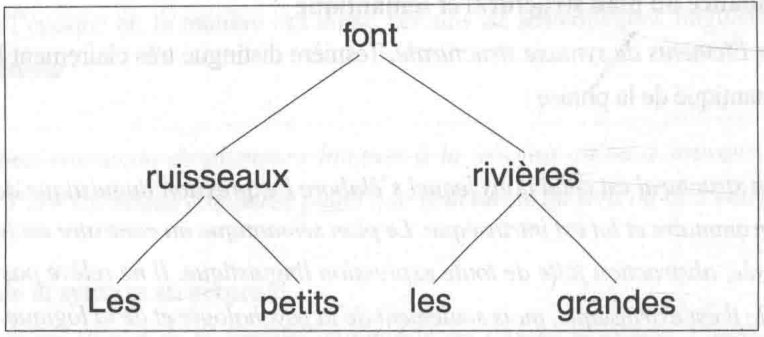
\includegraphics[width=.77\linewidth]{assets/ch10_stemma_ruisseaux.png}\end{center}
\end{minipage}\par\smallskip

Je présente également ci-dessous les stemmas des deux exemples déjà rencontrés plus haut :

\par\noindent\begin{minipage}{\linewidth}
\renewcommand{\thempfootnote}{校\arabic{editorialnote}}
\minititle{Stemma : \normalfont Le signal vert indique la voie libre.}
\begin{center}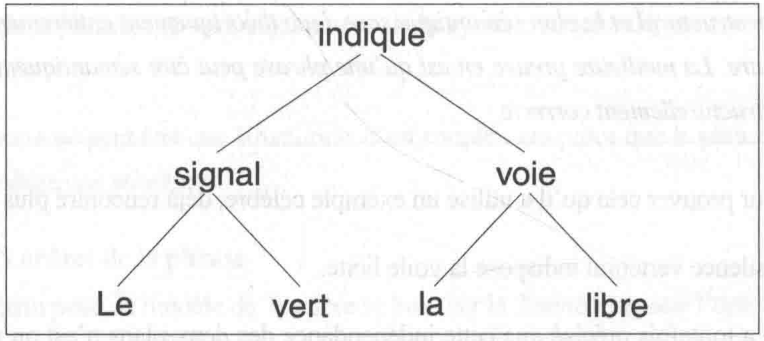
\includegraphics[width=.77\linewidth]{assets/ch10_stemma_signal.png}\end{center}
\end{minipage}\par\smallskip

\par\noindent\begin{minipage}{\linewidth}
\renewcommand{\thempfootnote}{校\arabic{editorialnote}}
\minititle{Stemma : \normalfont Le silence vertébral indispose la voile licite.}
\begin{center}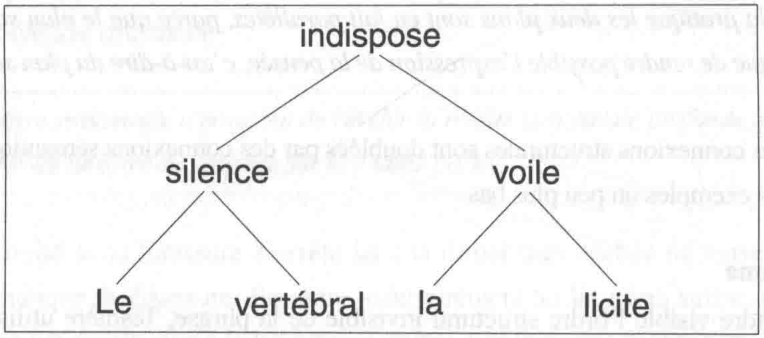
\includegraphics[width=.77\linewidth]{assets/ch10_stemma_silence.png}\end{center}
\end{minipage}\par\smallskip


\origpage{299}{285}
Comme c’est l’ordre structural (et non l’ordre linéaire) que le stemma donne à voir, remarquez qu’il ne suit pas l’ordre linéaire des mots sur la chaîne parlée. Ainsi, deux expressions différentes comme « les petits ruisseaux » et « les ruisseaux capricieux » seront représentées par le même stemma, avec « ruisseaux » comme terme supérieur et l’adjectif épithète comme terme inférieur :
\par\noindent\begin{minipage}{\linewidth}
\renewcommand{\thempfootnote}{校\arabic{editorialnote}}
\begin{center}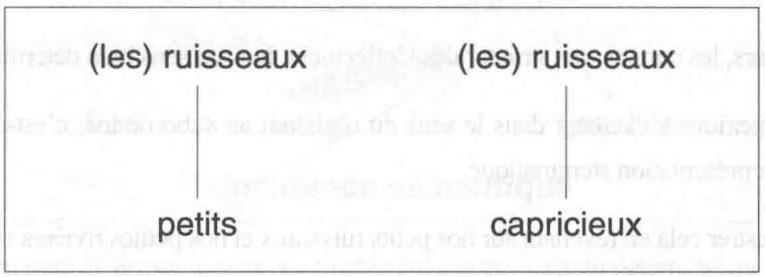
\includegraphics[width=.77\linewidth]{assets/ch10_stemma_adjectifs.png}\end{center}
\end{minipage}\par\smallskip


\subsection{Le modèle dépendanciel}
La syntaxe structurale de Tesnière, je l’ai dit, est plus connue sous le terme de grammaire de dépendance. L’idée centrale est qu’au sein de la phrase, les mots établissent des rapports de dépendance.
\begin{quote}\small\itshape
Les connexions structurales établissent entre les mots des rapports de dépendance.
\end{quote}
Nous avons déjà évoqué cela dans la première partie de ce chapitre. Tesnière qui a fait de cette notion de dépendance le cœur de son modèle dépendanciel, a identifié trois types de rapports de dépendance syntaxique :
\begin{quote}\small\itshape
Connexion, jonction et translation sont [...] les trois grands chefs sous lesquels viennent se ranger tous les faits de la syntaxe structurale.
\end{quote}

\minititle{\textcircled{\scriptsize 1} La connexion}
Définie comme le lien de dépendance entre un élément « régissant » (placé plus haut dans le stemma) et un élément « subordonné », la connexion correspond à la subordination dans la grammaire traditionnelle.
\begin{quote}\small\itshape
Chaque connexion unit en principe un terme supérieur à un terme inférieur.
\end{quote}
Le subordonné dépend du régissant et inversement, le régissant commande ou régit le subordonné. Ainsi, dans le stemma ci-dessous, le verbe « chante » est le régissant, et donc placé en position dominante, au dessus d’Alfred, qui est le subordonné. Le verbe, en effet, occupe chez Tesnière, la position la plus importante.

\par\noindent\begin{minipage}{\linewidth}
\renewcommand{\thempfootnote}{校\arabic{editorialnote}}
\minititle{Stemma : \normalfont Alfred chante.}
\origpage{300}{286}
\begin{center}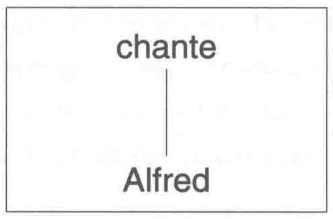
\includegraphics[width=.33\linewidth]{assets/ch10_stemma_alfred.png}\end{center}
\end{minipage}\par\smallskip

Par ailleurs, les connexions structurales s’effectuent dans un sens bien déterminé :
\begin{quote}
Les connexions s’exercent dans le sens du régissant au subordonné, c’est-à-dire de haut en bas dans la représentation stemmatique.
\end{quote}
Si on illustrer cela en revenant sur nos petits ruisseaux et nos petites rivières :\ednote{原文 Si on illustrer 是不完整的动词结构；按下文展示图示的语境，可校为 Si on illustre cela…（则还需补后件），或较自然地写 Illustrons cela…；也可能漏了 veut。本版不凭语感把拟补写进正文。}
\par\noindent\begin{minipage}{\linewidth}
\renewcommand{\thempfootnote}{校\arabic{editorialnote}}
\begin{center}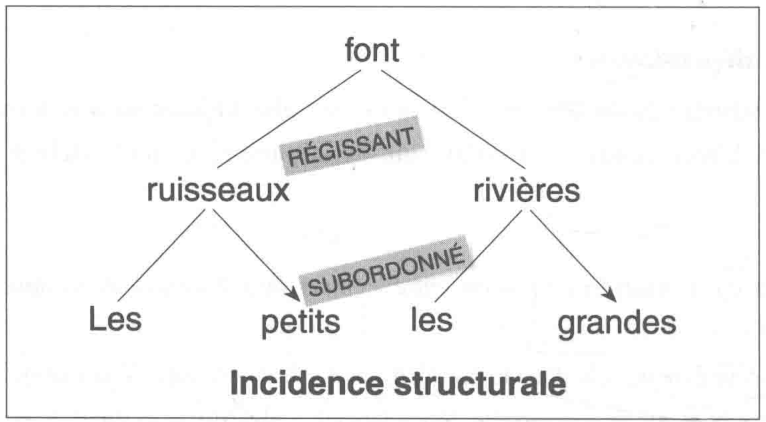
\includegraphics[width=.77\linewidth]{assets/ch10_incidence_structurale.png}\end{center}
\end{minipage}\par\smallskip

Dans le stemma ci-dessus, les deux flèches rouges indiquent ce mouvement qui va de haut en bas, du régissant au subordonné. Cela nous rappelle que sur le plan structural le régissant commande le noyau (appelé aussi \textit{nucléus}) inférieur, comme illustré dans le ci-dessous :\ednote{原文 dans le ci-dessous 疑漏 stemma 或 schéma。图中文字按原图保留；本底本为灰度扫描，无法重建所谓“红色”箭头的原色。}

\par\noindent\begin{minipage}{\linewidth}
\renewcommand{\thempfootnote}{校\arabic{editorialnote}}
\minititle{Stemma : \normalfont Mon ami parle.}
\begin{center}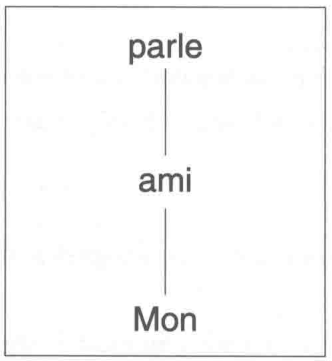
\includegraphics[width=.33\linewidth]{assets/ch10_stemma_ami.png}\end{center}
\end{minipage}\par\smallskip

Sur le plan sémantique, en revanche, c’est le subordonné qui détermine ou complète le régissant (\textit{nucléus} supérieur) : c’est l’illustration du principe d’autonomie et de parallélisme du plan structurel et sémantique dont je vous ai parlé un peu plus haut. Ainsi, au couple structural « régissant/subordonné » correspond un couple sémantique « déterminant/déterminé »,\ednote{按这句话前半及下一页汇总图，次序应为“régissant/subordonné 对应 déterminé/déterminant”：petits 在结构上从属于 ruisseaux，而在语义上限定 ruisseaux。原文将后一个二元组的顺序颠倒。} comme l’indique le schéma suivant :

\par\noindent\begin{minipage}{\linewidth}
\renewcommand{\thempfootnote}{校\arabic{editorialnote}}
\origpage{301}{287}
\begin{center}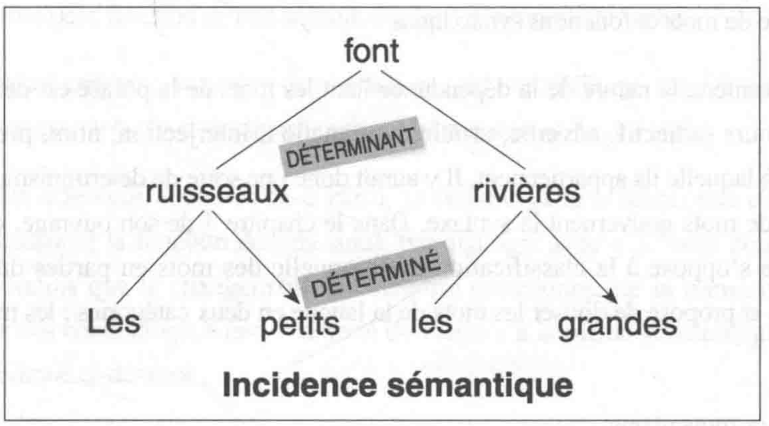
\includegraphics[width=.77\linewidth]{assets/ch10_incidence_semantique.png}\end{center}
\end{minipage}\par\smallskip

Vous avez noté, je pense, le sens des flèches rouges qui vont du déterminé au déterminant. On peut synthétiser tout cela à l’aide du schéma suivant :\ednote{本页第一图的语义箭头仍向下，déterminant/déterminé 标签也与本页下方汇总图相反。依作者给出的 petits « détermine » ruisseaux，语义方向应由下方 petits（déterminant）指向上方 ruisseaux（déterminé）；正文的 du déterminé au déterminant 同样颠倒。两张底本图均原样保存，不静默改图。}
\par\noindent\begin{minipage}{\linewidth}
\renewcommand{\thempfootnote}{校\arabic{editorialnote}}
\begin{center}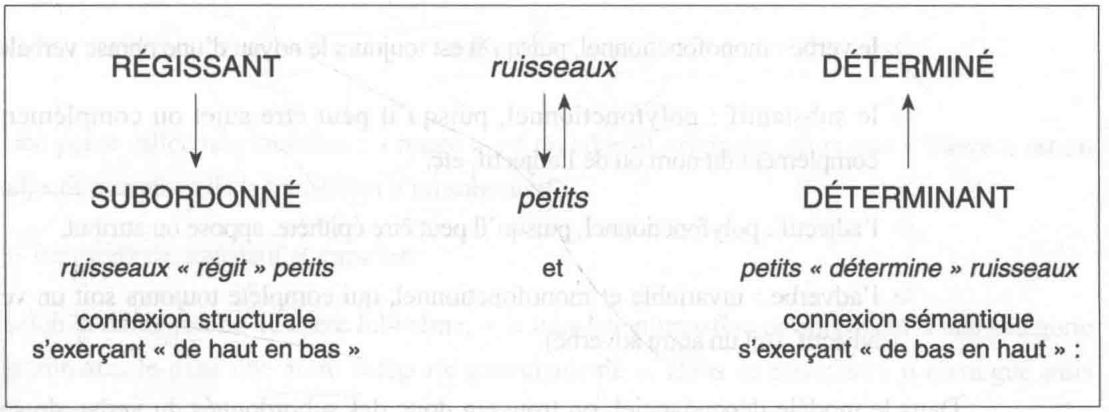
\includegraphics[width=\linewidth]{assets/ch10_structure_sens.png}\end{center}
\end{minipage}\par\smallskip


\minititle{\textcircled{\scriptsize 2} La translation}
Pour Tesnière, un mot peut assumer une fonction qui n’est pas prévue par sa nature en subissant une translation, opération qui le fait passer d’une catégorie grammaticale à une autre :
\begin{quote}\small\itshape
La translation consiste à transférer un mot plein d’une catégorie grammaticale dans une autre catégorie grammaticale, c’est-à-dire transformer une espèce de mot en une autre espèce de mot.
\end{quote}
Pour illustrer la notion de translation, Tesnière prend comme exemple « le livre de Pierre » et « le livre rouge », puis explique :
\begin{quote}\small\itshape
Dans le groupe « le livre de Pierre », le substantif « Pierre » devient syntaxiquement un adjectif épithète au même titre que rouge dans le livre rouge. Bien que non adjectif morphologiquement, il acquiert ainsi les caractéristiques syntaxiques de l’adjectif, c’est-à-dire la valeur adjectivale.
\end{quote}
C’est là un exemple de translation simple. Mais Tesnière a compliqué son modèle de façon à rendre compte du plus grand nombre possible de faits et a introduit des translations doubles, triples, quadruples, etc.

\origpage{302}{288}
\minititle{1. Classe de mots et fonctions syntaxiques}
Selon Tesnière, la nature de la dépendance liant les mots de la phrase est déterminée par la partie du discours (adjectif, adverbe, article, conjonction, interjection, nom, préposition, pronom et verbe.) à laquelle ils appartiennent. Il y aurait donc une sorte de déterminisme morphologique : les classes de mots gouvernent la syntaxe. Dans le chapitre 4 de son ouvrage, « Espèces de mots », Tesnière s’oppose à la classification traditionnelle des mots en parties du discours héritée de Priscien et propose de diviser les mots de la langue en deux catégories : les mots pleins et les mots vides.

\minititle{1) Les mots pleins}
Les mots pleins (appelés aussi « mots lexicaux ») sont les seuls à pouvoir faire l’objet d’une translation et à constituer un nœud, c’est-à-dire gouverner un autre élément. Tesnière distingue :
\begin{itemize}
\item le verbe : monofonctionnel, puisqu’il est toujours le noyau d’une phrase verbale.
\item le substantif : polyfonctionnel, puisqu’il peut être sujet ou complément du verbe, complément du nom ou de l’adjectif, etc.
\item l’adjectif : polyfonctionnel, puisqu’il peut être épithète, apposé ou attribut.
\item l’adverbe : invariable et monofonctionnel, qui complète toujours soit un verbe, soit un adjectif, soit un autre adverbe).
\end{itemize}
Dans le modèle dépendanciel, on trouvera donc des subordonnés du verbe, du substantif, de l’adjectif et de l’adverbe.

\minititle{2) Les mots vides}
Les mots vides, quant à eux, sont interdits de position de nœud : ils ne peuvent ni entrer en relation de dépendance, ni assumer les fonctions de régissant ou de subordonné. Ils comprennent ce que Tesnière appelle les « jonctifs » (conjonctions de coordination), et les « translatifs » (prépositions et conjonctions de subordination), auxquels il ajoute les articles et les pronoms.\ednote{“pronoms 一概属于不能占据节点的虚词”与本章后面的图示不一致：第291页 je crois…、第292页 Alfred a avoué qu’il a tué 的图中，人称代词 je、il 均为依存节点。至少应限定代词的种类与相应分析，不能把这句概括当作后面所有图示的通则。}

\minititle{2. Correspondance entre fonctions et catégories}
L’une des caractéristiques de la syntaxe de Tesnière est de chercher à établir une correspondance entre fonctions et catégories grammaticales : à chaque fonction correspond une seule catégorie, symbolisée par souci de formalisation par une lettre de l’alphabet :
\begin{itemize}
\item Verbe (I) : fonction de « nœud des nœuds », élément central de la proposition. Il ne dépend de rien et a deux types de dépendants : le substantif et l’adverbe.
\item Substantif (O) : fonction d’actant, élément dépendant du verbe.
\item Adjectif (A) : fonction adjectivale, élément dépendant d’un substantif.
\origpage{303}{289}
\item Adverbe (E) : fonction de circonstant, élément dépendant du verbe.
\end{itemize}
Pour revenir à présent à la notion de translation, tout mot plein qui assume une fonction autre que celle qui lui est attribuée ci-dessus change automatiquement de catégorie.

Ainsi, dans « Je vous demande de partir », le verbe « partir » fonctionne comme le COD de la phrase et assume la fonction de substantif, par analogie avec « Je vous demande \textit{une faveur} ». Notez toutefois que le changement de catégorie occasionné par la translation n’affecte pas la hiérarchie des connexions. Ainsi, « le livre de Pierre » a la même structure que « le livre rouge », comme indiqué ci-dessous :
\par\noindent\begin{minipage}{\linewidth}
\renewcommand{\thempfootnote}{校\arabic{editorialnote}}
\begin{center}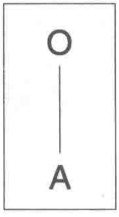
\includegraphics[width=.12\linewidth]{assets/ch10_categories_OA.png}\end{center}
\end{minipage}\par\smallskip

Une petite différence toutefois : « rouge » est un adjectif originaire, alors « Pierre » est un adjectif provenant de la translation d’un substantif.

\minititle{3. Transférende, translatif et transféré}
Selon la définition de Tesnière lui-même, « la translation transfère un mot plein d’une catégorie grammaticale dans une autre catégorie grammaticale ». Dans ce processus, il distingue trois éléments :
\begin{itemize}
\item Le transférende : le mot subissant la translation (la catégorie de départ)
\item Le transféré : le résultat de la translation (la catégorie d’aboutissement)
\item Le translatif : le mot vide par lequel s’effectue la translation.
\end{itemize}
\noindent\textbf{Ex :} Il a plu pendant un an.

Le \textit{transférende} « an » est un substantif \textit{transféré} en adverbe grâce au \textit{translatif} « pendant ». La translation est symbolisée par le signe >, comme suit :
\begin{center}Transférende > Transféré\end{center}
Pour Tesnière, le translatif est intranucléaire, c’est-à-dire qu’il forme avec le transférende un seul nucléus dont il n’est pas séparable, comme dans « le livre de Pierre ». Il s’oppose ainsi encore une fois à la grammaire traditionnelle qui considère que les prépositions et les conjonctions de subordination sont des mots de liaison, placés entre deux nucléus, et donc internucléaire.\ednote{原文 donc internucléaire 作复数主语的表述，应为 donc internucléaires。}

\minititle{4. Représentation graphique}
Si le changement de catégorie occasionné par la translation n’affecte pas la hiérarchie des\origcont{304}{290}connexions, dans le stemma, la translation dispose de sa propre représentation, symbolisée par le signe « $\tau$ » (la lettre grecque \textit{tau}). Au dessus de la barre horizontale du $\tau$, Tesnière place le transféré. Au-dessous de part et d’autre de la hampe du $\tau$, se trouvent le transférende et le translatif. Le crochet de la hampe du $\tau$ est tourné vers le translatif, comme suit :
\par\noindent\begin{minipage}{\linewidth}
\renewcommand{\thempfootnote}{校\arabic{editorialnote}}
\begin{center}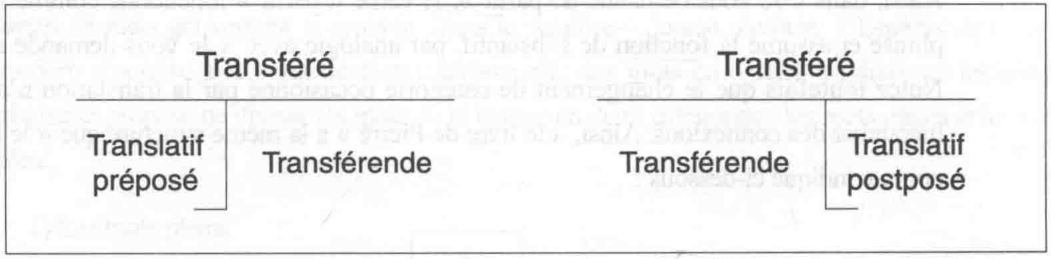
\includegraphics[width=\linewidth]{assets/ch10_tau_schema.png}\end{center}
\end{minipage}\par\smallskip

Je vous propose à présent d’illustrer tout cela à l’aide de quelques exemples pratiques, en allant du plus simple au plus compliqué :

\par\noindent\begin{minipage}{\linewidth}
\renewcommand{\thempfootnote}{校\arabic{editorialnote}}
\minititle{Stemma : \normalfont le livre de mon ami}
\begin{center}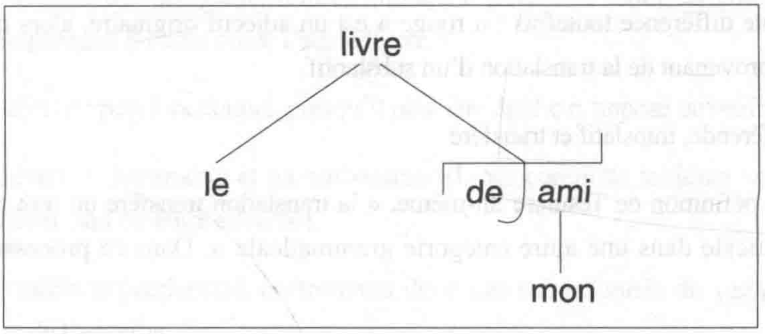
\includegraphics[width=.77\linewidth]{assets/ch10_livre_ami.png}\end{center}
\end{minipage}\par\smallskip

\par\noindent\begin{minipage}{\linewidth}
\renewcommand{\thempfootnote}{校\arabic{editorialnote}}
\minititle{Stemma : \normalfont la mode de parisienne > la mode de Paris\ednote{原图左侧为 la mode parisienne，图题 la mode de parisienne 多出 de，正文仍照录。此处是两个同功能表达的比较，不应将箭头读成派生方向：“Paris（名词）经 de 转成形容词性依存成分”，不是“parisienne 变成 Paris”。}}
\begin{center}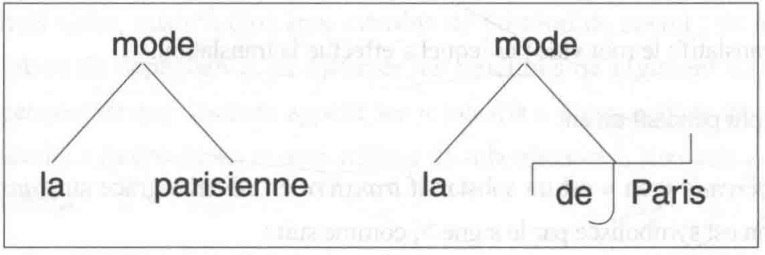
\includegraphics[width=.77\linewidth]{assets/ch10_mode_paris.png}\end{center}
\end{minipage}\par\smallskip

Dans l’exemple ci-dessous, pour vous aider, transférendre, translatif et transféré sont clairement indiqués.\ednote{正文 transférendre 应为 transférende。下图却把 parisienne 标为 TRANSFÉRENDE、Paris 标为 TRANSFÉRÉ，与前页三项定义相反：就 de Paris 而言，Paris 是输入项 transférende，de 是 translatif，形容词性成分 de Paris 才是转类结果 transféré；parisienne 是用于比较的原生形容词。原图标签保留。}
\par\noindent\begin{minipage}{\linewidth}
\renewcommand{\thempfootnote}{校\arabic{editorialnote}}
\begin{center}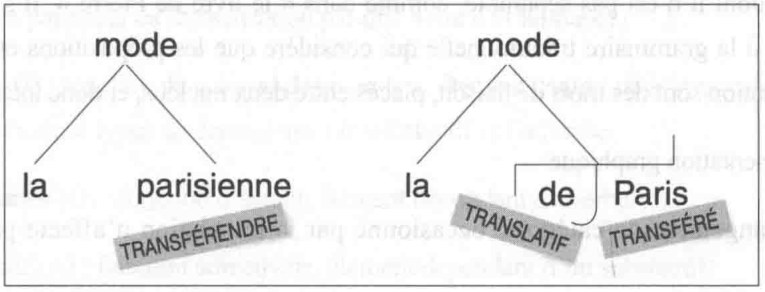
\includegraphics[width=.77\linewidth]{assets/ch10_mode_labels.png}\end{center}
\end{minipage}\par\smallskip


\par\noindent\begin{minipage}{\linewidth}
\renewcommand{\thempfootnote}{校\arabic{editorialnote}}
\origpage{305}{291}
\minititle{Stemma : \normalfont écrivez dans le livre de mon ami}
\begin{center}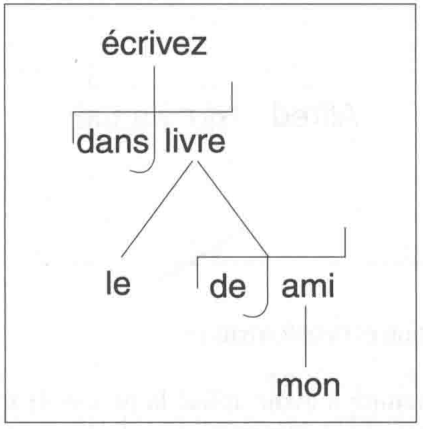
\includegraphics[width=.42\linewidth]{assets/ch10_ecrivez.png}\end{center}
\end{minipage}\par\smallskip

\par\noindent\begin{minipage}{\linewidth}
\renewcommand{\thempfootnote}{校\arabic{editorialnote}}
\minititle{Stemma : \normalfont le docteur qui a une barbe}
\begin{center}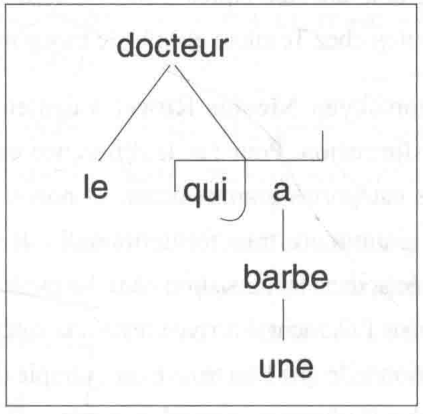
\includegraphics[width=.43\linewidth]{assets/ch10_docteur.png}\end{center}
\end{minipage}\par\smallskip

\par\noindent\begin{minipage}{\linewidth}
\renewcommand{\thempfootnote}{校\arabic{editorialnote}}
\minititle{Stemma : \normalfont je crois qu’Alfred frappe Bernard}
\begin{center}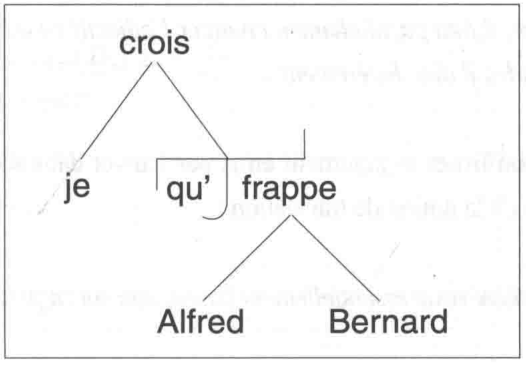
\includegraphics[width=.53\linewidth]{assets/ch10_je_crois.png}\end{center}
\end{minipage}\par\smallskip

\par\noindent\begin{minipage}{\linewidth}
\renewcommand{\thempfootnote}{校\arabic{editorialnote}}
\minititle{Stemma : \normalfont Alfred a avoué qu’il a tué}
\origpage{306}{292}
\begin{center}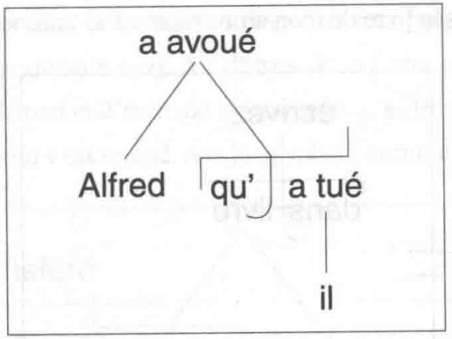
\includegraphics[width=.45\linewidth]{assets/ch10_alfred_avoue.png}\end{center}
\end{minipage}\par\smallskip


\minititle{5. Translation, transposition et transformation}
Tesnière n’est pas le premier à avoir utilisé la notion de translation : on la trouvait déjà, par exemple, chez \textbf{Charles Bally} qui l’appelait « transposition ». Mais c’est chez Tesnière que la translation est utilisée pour la première fois de façon systématique pour rendre compte d’un très grand nombre de faits grammaticaux. Après Tesnière, certains ont cru noter une forte similarité entre la notion de \textit{translation} chez Tesnière et celle de \textit{transformation} chez Chomsky.

Plus récemment, le chomskyen \textbf{Nicolas Ruwet} a également cherché à apprécier les liens entre translation et transformation. Pour lui, la différence essentielle est que les translations de Tesnière portent sur des catégories grammaticales et non sur des phrases entières, alors que la transformation dans la grammaire transformationnelle de Chomsky transforme des énoncés entiers. Pour être plus précis, dans la translation chez Tesnière, l’élément de départ de la translation est parfois une phrase, mais l’élément d’arrivée reste une catégorie grammaticale. Ce n’est que de façon absolument exceptionnelle que l’on trouve un exemple de transformation de phrase à phrase. Dans l’ouvrage de Tesnière, il n’y en qu’un seul exemple,\ednote{原文 il n’y en qu’un seul exemple 缺少 a，应为 il n’y en a qu’un seul exemple。} que je reproduis ci-dessous :
\begin{quote}\small\itshape
L’adverbe est au verbe ce que l’adjectif est au substantif. Il en résulte que, quand on change un substantif en verbe, il faut parallèlement changer l’adjectif en adverbe. Ainsi en français : « un dîner léger deviendra il dîne légèrement ».
\end{quote}
Tout cela semble confirmer le jugement émis par Ruwet dans son \textit{Introduction à la grammaire générative} à propos de la notion de translation :
\begin{quote}\small\itshape
La syntaxe de Tesnière reste essentiellement basée, non sur la phrase, mais sur le mot.
\end{quote}

\minititle{\textcircled{\scriptsize 3} La jonction}
Après la connexion et la translation, la jonction, définie comme la relation établie entre deux éléments de fonction équivalente, est le troisième des « grands chefs sous lesquels viennent se ranger tous les faits de la syntaxe structurale ».

\minititle{1. La notion de dédoublement}
La jonction correspond à la coordination de la grammaire traditionnelle. Prenons un exemple pour\origcont{307}{293}illustrer cette notion :

\par\noindent\begin{minipage}{\linewidth}
\renewcommand{\thempfootnote}{校\arabic{editorialnote}}
\minititle{Stemma : \normalfont Alfred et Bernard tombent.}
\begin{center}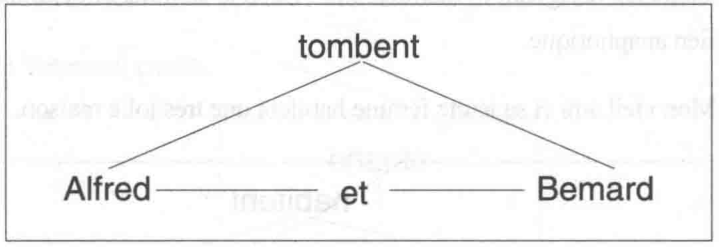
\includegraphics[width=.73\linewidth]{assets/ch10_alfred_bernard.png}\end{center}
\end{minipage}\par\smallskip

À proprement parler, il n’y a qu’un seul sujet, exprimé par deux termes coordonnés. Dans ce cas, Tesnière parle de « nucléus dédoublé » et précise que cette phrase comporte un seul sujet dédoublé.

\minititle{2. La jonction sans jonctif}
La jonction a la particularité de pouvoir être exprimée avec ou sans jonctif (conjonction de coordination dans la terminologie traditionnelle) :
\begin{quote}
Il peut y avoir jonction sans jonctif, c’est-à-dire que la fonction jonctive peut s’exercer sans qu’il y ait besoin d’un marquant pour l’indiquer : lat. veni, vidi, vici « je suis venu, j’ai vu, j’ai vaincu »
\end{quote}
Dans ce cas là, la jonction sans jonctif correspond à la juxtaposition de la terminologie traditionnelle, présentée dans le première partie de ce chapitre.\ednote{原文 le première partie 应为 la première partie。} Les jonctifs étant des mots vides, la jonction dans le stemma est représentée par un trait horizontal : le trait de jonction.

\minititle{3. La jonction de la phrase}
Si l’on peut coordonner des termes à l’intérieur d’une phrase, on peut aussi coordonner des phrases. Dans ce cas, on joint entre eux des verbes, comme suit :

\par\noindent\begin{minipage}{\linewidth}
\renewcommand{\thempfootnote}{校\arabic{editorialnote}}
\minititle{Stemma : \normalfont chante et Alfred Bernard crie\ednote{底本图题词序错乱；按图中两对支配关系，例句应为 Alfred chante et Bernard crie。图题仍保留原词序。}}
\begin{center}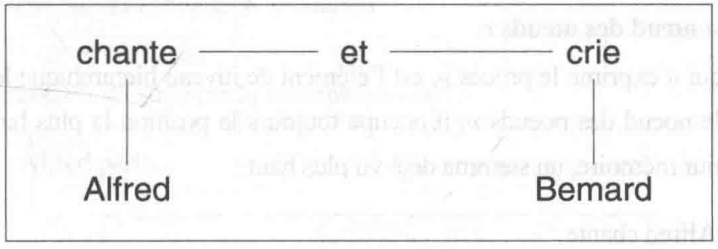
\includegraphics[width=.73\linewidth]{assets/ch10_chante_crie.png}\end{center}
\end{minipage}\par\smallskip

Une phrase comme « Alfred et Bernard tombent » résulte de l’addition de deux phrases : « Alfred tombe » et « Bernard tombe ». Autrement dit, dès qu’il y a dédoublement de nucléus subordonnés, on a affaire à des phrases elliptiques. Ce dédoublement à la fois de nucléus régissants et de nucléus subordonnés aboutit à des stemmas plus ou moins complexes avec croisement des traits de connexion : dans ce cas, Tesnière parle de \textit{plexus}.

\origpage{308}{294}
\minititle{4. Le cas de l’anaphore}
L’anaphore ne nous est pas inconnue : elle désigne, souvenez-vous, la relation sémantique existant entre deux éléments désignant la même réalité. Dans le stemma ci-dessous, « ami » et « sa » sont liés par un lien anaphorique.

\par\noindent\begin{minipage}{\linewidth}
\renewcommand{\thempfootnote}{校\arabic{editorialnote}}
\minititle{Stemma : \normalfont Mon vieil ami et sa jeune femme habitent une très jolie maison.}
\begin{center}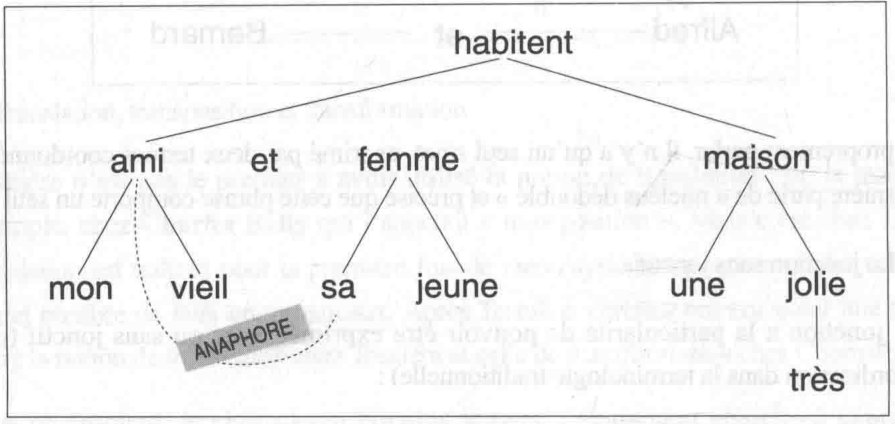
\includegraphics[width=.90\linewidth]{assets/ch10_anaphore.png}\end{center}
\end{minipage}\par\smallskip


\subsection{Le schéma actantiel}
En début de chapitre, nous avons présenté la notion de nœud verbal et rappelé l’importance du verbe dans la grammaire traditionnelle. Pour Tesnière, le nœud verbal constitue le cœur d’un « drame » mettant en scène des actants et des circonstants :
\begin{quote}\small\itshape
Le nœud verbal exprime tout un petit drame. Comme dans un drame en effet, il comporte obligatoirement un procès, et le plus souvent des acteurs et des circonstances. Transposés du plan de la réalité dramatique, sur celui de la syntaxe structurale, le procès, les acteurs et les circonstances deviennent respectivement le verbe, les actants et les circonstants.
\end{quote}

\minititle{\textcircled{\scriptsize 1} Le verbe, « nœud des nœuds »}
Le verbe, qui « exprime le procès », est l’élément de niveau hiérarchique le plus élevé : considéré comme « le nœud des nœuds », il occupe toujours la position la plus haute dans le stemma. Je rappelle, pour mémoire, un stemma déjà vu plus haut :

\par\noindent\begin{minipage}{\linewidth}
\renewcommand{\thempfootnote}{校\arabic{editorialnote}}
\minititle{Stemma : \normalfont Alfred chante.}
\begin{center}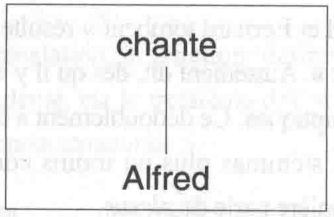
\includegraphics[width=.33\linewidth]{assets/ch10_alfred_rappel.png}\end{center}
\end{minipage}\par\smallskip


\origpage{309}{295}
\minititle{1. Du « nœud » au « nucléus »}
Si le verbe est « le nœud des nœuds », cela signifie qu’une phrase peut contenir plusieurs nœuds. La conception de Tesnière s’oppose ici encore à la grammaire traditionnelle.

\par\noindent\begin{minipage}{\linewidth}
\renewcommand{\thempfootnote}{校\arabic{editorialnote}}
\minititle{Stemma : \normalfont Votre ami chante.}
\begin{center}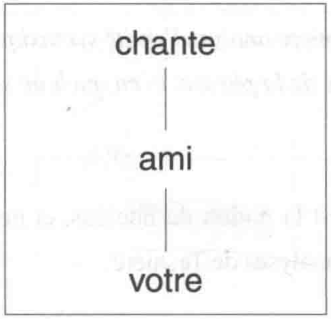
\includegraphics[width=.33\linewidth]{assets/ch10_votre_ami.png}\end{center}
\end{minipage}\par\smallskip

Dans l’exemple ci-dessus, et selon le modèle de Tesnière, il y a deux nœuds :
\begin{itemize}
\item « chante » forme un nœud \textit{verbal} avec « ami » et avec « votre ».
\item « ami » forme un nœud \textit{substantival} avec « votre ».
\end{itemize}
Le nœud, dans sa définition structurale, correspond au syntagme en grammaire traditionnelle. Pour s’écarter de cette dernière, Tesnière a introduit la notion de \textit{nucléus}.

\minititle{2. Première définition}
Noyau et nucléus ont le même sens littéral, mais Tesnière a introduit une différence conceptuelle entre eux :
\begin{quote}\small\itshape
Nous définissons le nucleus comme l’ensemble dans lequel viennent s’intégrer, outre le nœud structural proprement dit, tous les autres éléments dont le nœud est comme le support matériel, à commencer par les éléments sémantiques.
\end{quote}
Sa conception est illustrée par le stemma suivant :

\par\noindent\begin{minipage}{\linewidth}
\renewcommand{\thempfootnote}{校\arabic{editorialnote}}
\minititle{Stemma : \normalfont Alfred parle.}
\begin{center}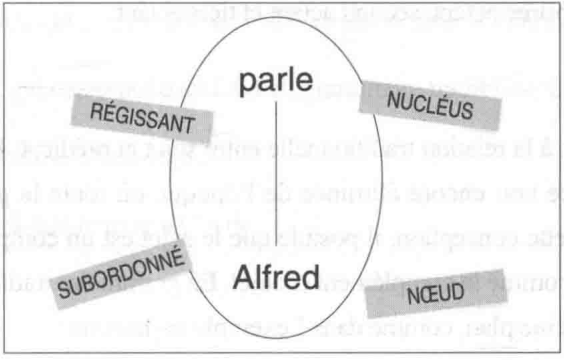
\includegraphics[width=.57\linewidth]{assets/ch10_nucleus_premiere.png}\end{center}
\end{minipage}\par\smallskip

\origpage{310}{296}
Tesnière considère le nucléus comme assumant une fonction à la fois structurale et sémantique.

\minititle{3. Deuxième définition}
Par un glissement progressif, Tesnière a donné au nucléus une autre définition. D’un \textit{ensemble} contenant des \textit{unités} structurales, il a été identifié à ces mêmes unités :
\begin{quote}\small\itshape
Le nucleus est donc en dernière analyse l’entité syntaxique élémentaire, le matériau fondamental de la charpente structurale de la phrase, et en quelque sorte la cellule constitutive qui en fait un organisme vivant.
\end{quote}
À partir de ce moment, c’est la notion de nucléus, et non plus celle de nœud, qui a été retenue comme point de départ des analyses de Tesnière.

\par\noindent\begin{minipage}{\linewidth}
\renewcommand{\thempfootnote}{校\arabic{editorialnote}}
\minititle{Stemma : \normalfont Mon ami parle.}
\begin{center}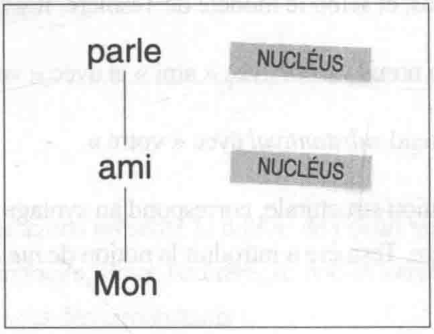
\includegraphics[width=.44\linewidth]{assets/ch10_nucleus_deuxieme.png}\end{center}
\end{minipage}\par\smallskip

Quant à l’utilisation des métaphores issues de la biologie (\textit{nucleus}, cellule, organisme vivant), elle ne nous surprendra pas : rappelons que, pour Tesnière, construire une phrase, « c’est mettre un peu de vie dans une masse amorphe de mots. »

\minititle{\textcircled{\scriptsize 2} Les actants}
Après le verbe, place aux acteurs du « drame », les actants, définis par Tesnière comme :
\begin{quote}\small\itshape
Les êtres ou les choses qui, à un titre quelconque et de quelque façon que ce soit, infime au titre de simples figurants et de la façon la plus passive, participent au procès.
\end{quote}
Ils se divisent en prime actant, second actant et tiers actant.

\minititle{1. Prime actant}
Tesnière s’oppose à la relation traditionnelle entre sujet et prédicat. Pour lui, cette opposition n’est qu’une survivance non encore éliminée de l’époque où toute la grammaire était fondée sur la logique. Contre cette conception, il postule que le sujet est un complément comme les autres, qui dépend du verbe comme le complément d’objet. En grammaire traditionnelle, sujet et prédicat sont représentés sur même plan,\ednote{原文 sur même plan 缺少定冠词，通常应为 sur le même plan。} comme dans l’exemple ci-dessous :
\par\noindent\begin{minipage}{\linewidth}
\renewcommand{\thempfootnote}{校\arabic{editorialnote}}
\origpage{311}{297}
\begin{center}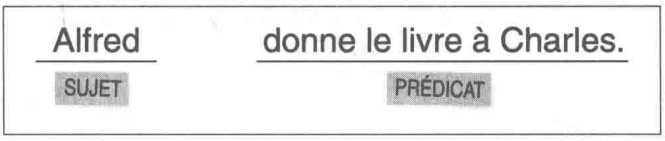
\includegraphics[width=.67\linewidth]{assets/ch10_sujet_predicat.png}\end{center}
\end{minipage}\par\smallskip

Chez Tesnière, le prime actant est régi par le verbe, comme dans « Alfred dort ».
\par\noindent\begin{minipage}{\linewidth}
\renewcommand{\thempfootnote}{校\arabic{editorialnote}}
\begin{center}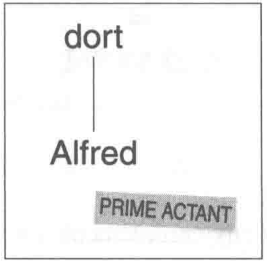
\includegraphics[width=.27\linewidth]{assets/ch10_alfred_dort.png}\end{center}
\end{minipage}\par\smallskip

En conséquence, le prime actant se trouve représenté sur le stemma au même niveau que le complément d’objet. L’exemple ci-dessous illustre pour un même exemple la démarche de Tesnière à la grammaire traditionnelle :\ednote{原文 la démarche de Tesnière à la grammaire traditionnelle 缺少表达比较或对照的连接成分；可拟读为 oppose la démarche de Tesnière à celle de la grammaire traditionnelle，但此处仅据上下文拟校，不视作已经恢复的原句。}

\par\noindent\begin{minipage}{\linewidth}
\renewcommand{\thempfootnote}{校\arabic{editorialnote}}
\minititle{Stemma : \normalfont Alfred frappe Bernard.}
\begin{center}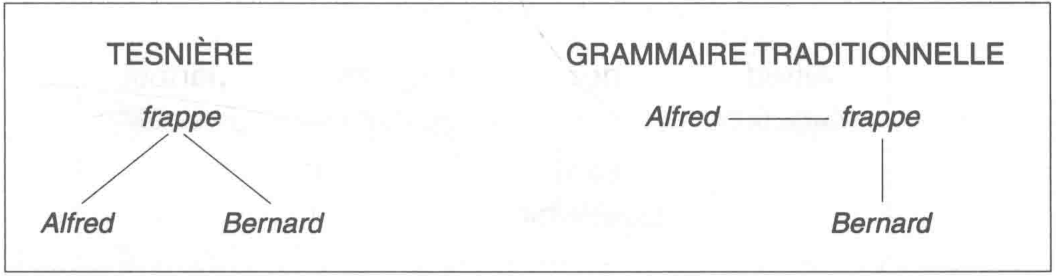
\includegraphics[width=\linewidth]{assets/ch10_frappe_comparaison.png}\end{center}
\end{minipage}\par\smallskip

Tesnière prend soin de différencier encore une fois le plan syntaxique du plan sémantique : c’est du point de vue structural, et non du point de vue sémantique, que le sujet est un complément comme les autres.

\minititle{2. Second actant et tiers actant}
Le sujet, bien que dépendant du verbe, occupe une place dominante par rapport aux autres actants, à savoir :
\begin{itemize}
\item le second actant, qui correspond au COD en grammaire traditionnelle.
\item le tiers actant, qui correspond au COI en grammaire traditionnelle.
\end{itemize}
Illustrons cela à l’aide d’un exemple.

\par\noindent\begin{minipage}{\linewidth}
\renewcommand{\thempfootnote}{校\arabic{editorialnote}}
\minititle{Stemma : \normalfont Alfred donne le livre à Charles.}
\origpage{312}{298}
\begin{center}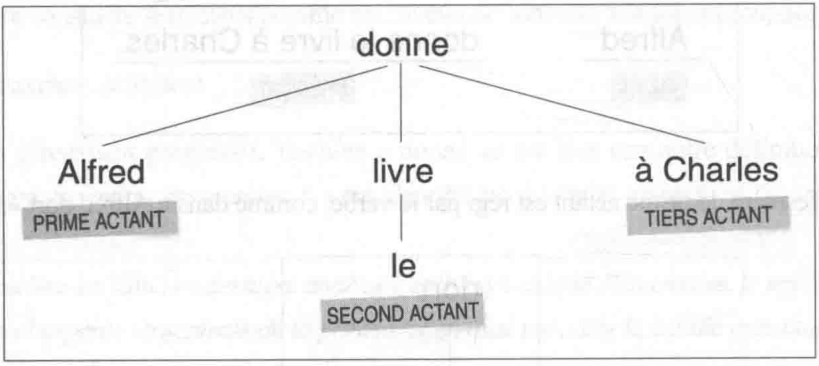
\includegraphics[width=.83\linewidth]{assets/ch10_trois_actants.png}\end{center}
\end{minipage}\par\smallskip


\minititle{\textcircled{\scriptsize 3} Les circonstants}
Les circonstants correspondent aux compléments circonstanciels de la grammaire traditionnelle, et expriment les circonstances (temps, lieu, manière, etc.) dans lesquelles se déroule « le procès », comme illustré ci-dessous :

\par\noindent\begin{minipage}{\linewidth}
\renewcommand{\thempfootnote}{校\arabic{editorialnote}}
\minititle{Stemma : \normalfont Alfred fourre son nez de partout.\ednote{图题与图中词项不一致：图有 toujours 和 partout，没有 de。按图中词项顺序还原应为 Alfred fourre toujours son nez partout。保留原图题，不把二者静默统一。}}
\begin{center}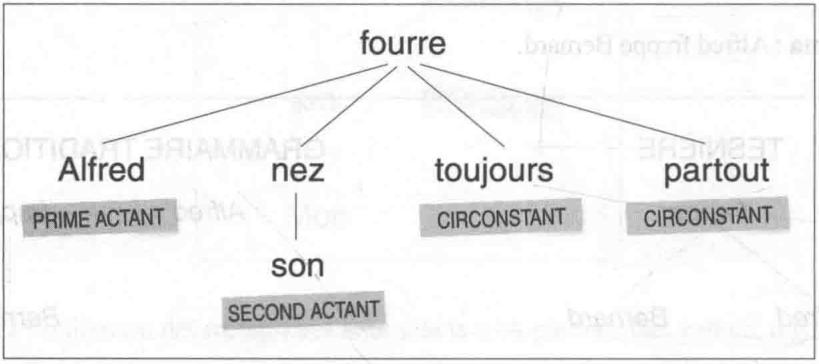
\includegraphics[width=.83\linewidth]{assets/ch10_circonstants.png}\end{center}
\end{minipage}\par\smallskip

Dans l’exemple ci-dessus, vous avez sûrement reconnu un complément circonstanciel de temps et un complément circonstanciel de lieu.

\subsection{La notion de valence}
La grammaire traditionnelle nous apprend que certains verbes n’ont aucun complément d’objet (mourir), que certains en ont un (manger), et que d’autres en ont deux (donner). Dans la terminologie tesnièrienne, on dira que les verbes peuvent régir zéro, un, deux, ou trois actants. Le fait de régir (ou pas) un certain nombre d’actants est une propriété individuelle de chaque verbe que Tesnière appelle « valence », terme venu tout droit de la chimie.

\minititle{\textcircled{\scriptsize 1} L’origine de la notion}
En chimie, la valence d’un élément est le nombre maximal de liaisons qu’il peut former avec d’autres éléments. Un élément « univalent » est un élément chimique qui formera des molécules en ne se liant qu’une seule fois. Les éléments « bivalents », « trivalents » voire « tétravalents » pourront respectivement s’associer avec deux, trois ou quatre atomes d’un élément univalent : c’est le cas par exemple du méthane (CH4) où le carbone, qui a une valence quadruple, est lié à quatre\origcont{313}{299}hydrogènes univalents, d’où son nom de CH4.\ednote{此处 CH4 是甲烷的分子式，不是其名称；宜作 d’où sa formule CH\textsubscript{4}。原书正文中的数字 4 按底本保留，规范化学式在本注中以下标表示。}

\minititle{\textcircled{\scriptsize 2} La valence des verbes}
Tesnière classe les verbes en fonction du nombre d’actants qu’ils peuvent avoir, et distingue ainsi :
\begin{itemize}
\item les verbes avalents : verbes impersonnels
\item les verbes monovalents : verbes intransitifs
\item les verbes divalents : verbes transitifs
\item les verbes trivalents : verbes transitifs doubles
\end{itemize}

\minititle{1. Les verbes avalents}
Les verbes avalents sont des verbes sans actant dont la valence est nulle. Il s’agit des verbes impersonnels comme « il pleut », ou « il faut », etc.\ednote{非人称形式不自动意味着零配价。falloir 可以带不定式或命题性补足成分，如 Il faut partir、Il faut que tu partes；因此不能仅因形式主语 il 不指称就把该动词所有用法一概归为 avalent。本注只指出原概括过强，不替换正文的理论框架；参见\ecite{53}第189页的非人称动词补足语表；配价判断是据这些构式作出的辨析。} On dira de ces verbes qu’ils ont une valence zéro.

\par\noindent\begin{minipage}{\linewidth}
\renewcommand{\thempfootnote}{校\arabic{editorialnote}}
\minititle{Stemma : \normalfont Il pleut.}
\begin{center}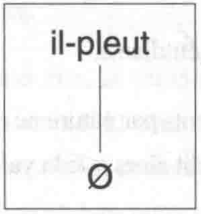
\includegraphics[width=.20\linewidth]{assets/ch10_il_pleut.png}\end{center}
\end{minipage}\par\smallskip


\minititle{2. Les verbes monovalents}
Comme leur nom l’indique, les verbes monovalents ne régissent qu’un seul actant. Si l’on s’en tient strictement à Tesnière, les verbes d’état comme « être », « paraître » sont monovalents en ce sens qu’ils ne comportent qu’un (prime) actant auquel l’énonciateur attribue une propriété.
\begin{quote}\textbf{Ex :} L’étudiante paraît passionnée.\end{quote}
Certains verbes « de processus » peuvent être aussi monovalents lorsque l’agent n’enclenche pas le procès de façon volontaire.
\begin{quote}
\textbf{Ex :} La neige tombe.\par
Le soleil brille.\par
Les élèves baillent.
\end{quote}
Il existe aussi des verbes d’action n’impliquant qu’un seul actant. Dans ce cas là, l’actant est un agent doté d’intentionnalité :
\begin{quote}\textbf{Ex :} Papa mange.\end{quote}
\origpage{314}{300}
\begin{quote}Les enfants crient.\end{quote}
Les verbes monovalents, de valence 1, correspondent aux verbes intransitifs la grammaire traditionnelle.\ednote{原文 verbes intransitifs la grammaire traditionnelle 缺少 de，通常应为 verbes intransitifs de la grammaire traditionnelle。} Les verbes transitifs, quant à eux, sont bivalents ou trivalents, comme nous allons le voir ci-dessous.

\minititle{3. Les verbes bivalents}
Les verbes bivalents sont les verbes à deux actants (de « valence 2 ») qui font transiter le procès d’un agent/acteur, volontaire ou non, vers un patient/objet, qui subit ce procès :
\begin{quote}
\textbf{Ex :} Le footballeur frappe le ballon.\par
Le soleil brûle ma peau.
\end{quote}

\minititle{4. Les verbes trivalents}
Les verbes trivalents (de « valence 3 ») permettent la transition d’un objet/patient vers un bénéficiaire (ou un détrimentaire) à travers un agent/acteur.
\begin{quote}
\textbf{Ex :} Pierre offre un cadeau à sa femme.\par
Le professeur fait cours à ses étudiants.
\end{quote}
Dans certains cas, les verbes trivalents par nature ne régissent que deux actants en situation d’énoncé (« Le professeur fait cours ») : on dit alors que la valence du verbe est « non saturée ».

\minititle{\textcircled{\scriptsize 3} La valence des noms}
Certains substantifs sont créés par la nominalisation d’actions verbales : la notion de valence leur est donc applicable. Prenons un exemple :
\begin{quote}\textbf{Ex :} L’invasion de la Grèce par les Barbares.\end{quote}
« Invasion » est la nominalisation du verbe « envahir ». Or, ce verbe est bivalent, que ce soit à l’actif comme au passif :
\begin{quote}
\textbf{Ex :} Les Barbares (\textit{prime actant}) ont envahi la Grèce (\textit{second actant}).\par
La Grèce (\textit{patient}) a été envahie par les Barbares (\textit{agent}).
\end{quote}
La structure nominalisée « invasion » est donc bivalente.

\minititle{\textcircled{\scriptsize 4} La valence des adjectifs}
Certains adjectifs ont une valence non nulle et disposent d’un complément, appelé complément de l’adjectif, comme dans l’exemple ci-dessous :
\begin{quote}\textbf{Ex :} Il est différent de moi.\end{quote}
Dans cet exemple, « de moi » est le complément de l’adjectif « différent ». Le complément de\origcont{315}{301}l’adjectif est généralement introduit par les jonctifs (prépositions) suivants :\ednote{此处 jonctifs 与本章此前的术语定义冲突：原书 p.293 把 jonctif 对应于并列连词，而此处列举 à、de、pour 等介词。就此句而言可直接改称 prépositions；按本章 translation 的分析，介词所起的作用应与 translatif 区分说明，而不宜与 jonctif 混同。} à, de, pour, contre, envers, avec, en, sur, etc.
\begin{quote}
\textbf{Ex :} Il est semblable à lui-même.\par
Il est fier de ses enfants.\par
Il est taillé pour l’aventure.\par
Il est furieux contre cette décision.\par
Il est généreux envers ses parents.\par
Il est aimable avec tout le monde.\par
Il est doué en linguistique.\par
Le professeur est intarissable sur la grammaire de dépendance de Tesnière
\end{quote}
Pour conclure en quelques mots sur Tesnière, retenez qu’il a intégré des éléments sémantiques dans un modèle originellement structural : la phrase, pour lui, est donc un composé complexe de relations structurales et sémantiques.

Pour cette raison, à l’époque moderne, la sémantique et la sémiologie ont repris des notions tesnièriennes : c’est le cas par exemple du sémiologue \textbf{Algirdas Julien Greimas} qui, dans sa \textit{Sémantique structurale} (1966) a repris les notions d’actant et de modèle actanciel. Nous verrons justement cela (et bien d’autres choses) dans notre prochain chapitre, consacré à la sémantique.

\section*{Exercices}
\phantomsection\addcontentsline{toc}{section}{Exercices}
\minititle{I. Les phrases suivantes sont-elles formées par coordination, juxtaposition ou subordination ?}
\begin{keybox}
\begin{enumerate}[label=\arabic*.,leftmargin=1.6em]
\item Il arrive que les routes soient recouvertes de neige en hiver.
\item Julie est allée voir sa grand mère, elle a fait des courses, elle a sorti le chien.
\item Mon petit cousin ne croit pas que le Père Noël existe.
\item Le chien a traversé la route et s’est fait écraser.
\item Pierre s’est perdu : il avait oublié son GPS.
\item Je pense donc je suis.
\item L’enfant a glissé, s’est étalé de tout son long, s’est égratigné les genoux.
\end{enumerate}
\end{keybox}
\origpage{316}{302}
\begin{keybox}
\begin{enumerate}[label=\arabic*.,start=8,leftmargin=1.6em]
\item Les électeurs qui se sont abstenus ont eu tort.
\item Parce que je suis malade, je n’ai pas faim.
\item Il est au régime, il ne mange ni oeufs ni poisson.
\item Je suis venu, j’ai vu, j’ai vaincu.
\item Je pense, donc je suis.
\item On voit bien que tout est à recommencer.
\item Si je tombe, je t’entraîne avec moi.
\item Le jeu auquel je participe est très intéressant.
\item Elle est arrivée quand je partais.
\end{enumerate}
\end{keybox}

\Needspace{18\baselineskip}
\minititle{II. Réalisez les stemmas des phrases suivantes :}
\begin{keybox}
\renewcommand{\thempfootnote}{校\arabic{editorialnote}}
\begin{enumerate}[label=\arabic*.,leftmargin=1.6em]
\item Écrire lisiblement
\item Le postier remet une lettre à ma voisine
\item Le chien du maître
\item Les bons comptes font les bons amis
\item Alfred mange une pomme voisin et sa femme ont acheté une belle maison\ednote{底本此题显见串行或缺文：Alfred mange une pomme 与 voisin et sa femme ont acheté une belle maison 不能按现有词序组成一个通常的句子。可能是两个例句误接，但后一部分的限定词无法仅据底本确证；保留原题，不擅自拆题或补造确定版本。本注不提供习题答案。}
\item Je crois que ce chapitre est fini.
\end{enumerate}
\end{keybox}

\section*{Pour aller plus loin}
\phantomsection\addcontentsline{toc}{section}{Pour aller plus loin}
\begingroup\small
\begin{description}[font=\normalfont,leftmargin=1.3em,labelindent=0pt,style=nextline]
\item[] RUWET (Nicolas). \textit{Introduction à la grammaire générative}. Paris, Plon, 1967.
\item[] TELLIER (Christine). Éléments de syntaxe du français. Méthodes d’analyse en grammaire générative, Montréal, Gaëtan Morin Éditeur, 2003.
\item[] TESNIÈRE (Lucien). \textit{Éléments de syntaxe structurale}. Paris, Klincksieck, 1959.
\item[] TESNIÈRE (Lucien). \textit{Esquisse d’une syntaxe structurale}. Paris, Klincksieck, 1953.
\end{description}
\endgroup

\clearpage
\origpage{317}{303}
\section*{Glossaire}
\phantomsection\addcontentsline{toc}{section}{Glossaire}
\gloss{acceptabilité 可接受性}{语言学中以某一语言变体为母语的人判断某一语言项在该变体中存在的可能性。}
\gloss{coordination 并列连接}{由并列连词连接对等或同级的语言单位。}
\gloss{énoncé 称述}{参见第 12 章。}
\gloss{phrase 句子}{语法中最大的语法结构单位，不同的词类和不同的语法结构在这个单位里起不同作用。}
\gloss{phrase complexe 复杂句，复句}{除主句外还包含一个或一个以上从属从句的句子。\ednote{这条释义只覆盖主从复句，而本章原书 pp.272–275 也把并列连接、并置的多小句句子放在 phrase complexe 范围内。为与本章定义一致，应把并列和并置的情形一并包括，而不能要求每个复句都含从属从句。}}
\gloss{phrase simple 简单句，单句}{只有一个述谓的句子称为单句。}
\gloss{subordination 从属连接}{由从属连词把独立分句和从属分句连接起来。\ednote{“由从属连词”限制过窄：本章 p.274 已列出由关系代词连接的从属结构，并举出含不定式的嵌入结构。宜释为一个分句在结构上依附于另一分句或其组成部分的连接关系；标记不限于从属连词。}}
